\documentclass[twoside, 12pt]{article}
\usepackage{amsmath}
\usepackage{lipsum} % Package to generate dummy text throughout this template
\usepackage[english]{isodate}% http://ctan.org/pkg/isodate
\usepackage{pgfgantt}
\usepackage[show]{ed}
\setlength{\parindent}{0pt}
\usepackage[sc]{mathpazo} % Use the Palatino font
\usepackage[T1]{fontenc} % Use 8-bit encoding that has 256 glyphs
\linespread{1.2} % Line spacing - Palatino needs more space between lines
\usepackage{microtype} % Slightly tweak font spacing for aesthetics
\usepackage{minted}
\usepackage{enumitem}
\usepackage[section]{placeins}
\usepackage{nameref}
\usemintedstyle{autumn}
\usepackage[hmarginratio=1:1,top=32mm,left=25mm,right=25mm,columnsep=18pt,bottom=27mm]{geometry} % Document margins
\usepackage{multicol} % Used for the two-column layout of the document
\usepackage[hang, small,labelfont=bf,up,textfont=it,up]{caption} % Custom captions under/above floats in tables or figures
\usepackage{booktabs} % Horizontal rules in tables
\usepackage{float} % Required for tables and figures in the multi-column environment - they need to be placed in specific locations with the [H] (e.g. \begin{table}[H])
\usepackage{hyperref} % For hyperlinks in the PDF
\usepackage{xspace}
\usepackage{lettrine} % The lettrine is the first enlarged letter at the beginning of the text
\usepackage{paralist} % Used for the compactitem environment which makes bullet points with less space between them
\usepackage{etoolbox}
\usepackage{eurosym}
\patchcmd{\thebibliography}{\section*{\refname}}{}{}{}
\usepackage{abstract} % Allows abstract customization
\renewcommand{\abstractnamefont}{\normalfont\bfseries} % Set the "Abstract" text to bold
\renewcommand{\abstracttextfont}{\normalfont\small\itshape} % Set the abstract itself to small italic text

\usepackage{titlesec} % Allows customization of titles
%\renewcommand\thesection{\Roman{section}} % Roman numerals for the sections
%\renewcommand\thesubsection{\Roman{subsection}} % Roman numerals for subsections
\titleformat{\section}[block]{\large\scshape\centering\bfseries}{\thesection.}{1em}{} % Change the look of the section titles
\titleformat{\subsection}[block]{\large\scshape}{\thesubsection.}{1em}{} % Change the look of the section titles
\usepackage{cite}
\usepackage{fancyhdr} % Headers and footers
\pagestyle{fancy} % All pages have headers and footers
\fancyhead{} % Blank out the default header
\fancyfoot{} % Blank out the default footer
\fancyhead[C]{Naomi Pentrel $\cdot$ \href{mailto:n.pentrel@jacobs-university.de}{n.pentrel@jacobs-university.de} $\cdot$ \today} % Custom header text
\fancyfoot[RO,LE]{\thepage} % Custom footer text
\usepackage{graphicx}
\usepackage{wrapfig}
\usepackage[]{natbib}
\usepackage{tocloft}
\renewcommand*{\figureautorefname}{figure}
\def\stex{\texorpdfstring{\raisebox{-.5ex}S\kern-.5ex\TeX}{sTeX}\xspace}
\def\sTeX{\stex}

\usepackage{quoting}
\quotingsetup{vskip=50pt}

%\usepackage{csquotes}
%\MakeOuterQuote{"}

\hypersetup{
    bookmarks=true,
    unicode=false,
    pdftoolbar=true,
    pdfmenubar=true,
    pdffitwindow=false,
    pdfstartview={FitH},
    pdftitle={My title},
    pdfauthor={Author},
    pdfsubject={Subject},
    pdfcreator={Creator},
    pdfproducer={Producer},
    pdfkeywords={keyword1} {key2} {key3},
    pdfnewwindow=true,
    colorlinks=false,
    %linkcolor=red,
    %citecolor=green,
    %filecolor=magenta,
    %urlcolor=cyan
    pdfborder={0 0 0},
}


\usepackage{caption}
\usepackage{subcaption}
\usepackage[section]{placeins}
\usepackage{qtree}
\usepackage{gensymb}

\usepackage{setspace}

\usepackage{color}

%\doublespacing
% or:
%\onehalfspacing

%\renewcommand\cftchapafterpnum{\vskip10pt}
%\renewcommand\cftsecafterpnum{\vskip15pt}

%----------------------------------------------------------------------------------------
%	TITLE SECTION
%----------------------------------------------------------------------------------------

\title{\vspace{-15mm}\fontsize{24pt}{10pt}\selectfont\textbf{// All comments are NOT created equal}} % Article title


\newenvironment{myfont}{\fontfamily{\sfdefault}\selectfont}{\par}

%----------------------------------------------------------------------------------------
% Macros
%----------------------------------------------------------------------------------------
\newcommand{\sys}{\textsc{RPresentation}\xspace}

%----------------------------------------------------------------------------------------

\begin{document}
\thispagestyle{empty}
\pagenumbering{roman}
\begin{flushright}
    
\includegraphics[scale=1.0]{assets/Logo}
  \end{flushright}
  \vspace{20mm}
  \begin{center}
    \huge
    \textbf{The Combination of Spatial Narrative and Semantic Closeness to Derive Visualizations of Information Graphs}
  \end{center}
  \vspace*{4mm}
  \begin{center}
   \Large by
  \end{center}
  \vspace*{4mm}
  \begin{center}
    \Large
    \textbf{Naomi Pentrel}
  \end{center}
  \vspace*{20mm}
  \begin{center}
    \large
    Bachelor Thesis in Computer Science
  \end{center}
  \vfill
  \begin{flushright}
    \large
    \begin{tabular}{l}
      
      \hline
      Prof. Dr. Michael Kohlhase \\
      \\
    \end{tabular}
  \end{flushright}
  \vspace*{8mm}
  \begin{flushleft}
    \large
    Date of Submission: \today \\
    \rule{\textwidth}{1pt}
  \end{flushleft}
  \begin{center}
    \Large Jacobs University Bremen - School of Engineering and Science
  \end{center}

\newpage
\noindent
With my signature, I certify that this thesis has been written by me using only the indicated resources and materials. Where I have presented data and results, the data and results are complete, genuine, and have been obtained by me unless otherwise acknowledged; where my results derive from computer programs, these computer programs have been written by me unless otherwise acknowledged. I further confirm that this thesis has not been submitted, either in part or as a whole, for any other academic degree at this or another institution.

  \vspace{20mm}

    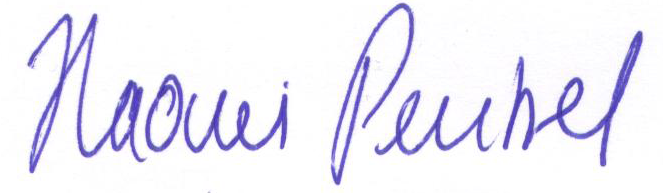
\includegraphics[scale=0.2]{assets/Signature}
 \hfill Bremen, \today
  
\newpage

\thispagestyle{fancy} % All pages have headers and footers

%----------------------------------------------------------------------------------------
%	ARTICLE CONTENTS
%----------------------------------------------------------------------------------------

 \section*{Abstract}
 \label{sec:abstract}
Visualization of knowledge is important to foster learning. To optimize the visualization of information and its interdependencies, we focus on identifying ways to present information without loosing context. The following research takes an existing annotated corpus and presents its contents in an interactive way that allows the audience to see the dependencies of the covered topics. This form of presenting knowledge enables users to interactively examine materials that are related to the topics the audience is interested in.\\

Taking the typical lecture as an example, it is often the case that, especially towards the end of the semester, students have difficulties remembering earlier topics. When a new topic is introduced it would be ideal to have a simple way to find dependencies and present students with an easy way to catch up.\\

The OMDoc (\textbf{O}pen \textbf{M}athematical \textbf{Doc}uments) format \cite{Kohlhase:OMDoc1.2} is a content markup scheme for mathematical documents. Using OMDoc, the implemented system can present different pieces of mathematical concepts in an interactive and connected way that allows students to learn the concepts the current topic depends on, should they need to refresh their memories. Along these lines it examines if and how spatial narrative and semantic closeness can be combined to foster learning. This approach to presenting learning materials changes how we interact with course material which will allow students to learn better. Ultimately, this research is applicable to almost all areas in which knowledge needs to be transferred.\\ 

\newpage
\tableofcontents

\clearpage

\newpage
\thispagestyle{empty}
\topskip0pt
\vspace*{\fill}
\begin{center}
\textsc{Aut viam inveniam aut faciam}\\

\vspace*{1cm}

\textit{(I'll either find a path or make one)}\\

\vspace*{4cm}

\centering

\begin{quoting}
\begin{center}
\noindent
\textit{At this point, I would like to thank Prof. Dr. Michael Kohlhase for being an inspiring and helpful supervisor. Additionally, I would like to thank Mihnea Iancu and Tom Wiesing for aiding me in my research project.\\}
\end{center}
\end{quoting}

\vspace*{\fill}
\end{center}

\newpage
\pagenumbering{arabic}

\section{Introduction \& Motivation}
\label{sec:introduction}

\begin{wrapfigure}{r}{0.3\textwidth}
\vspace{-28pt}
  \begin{center}
  \fbox{
    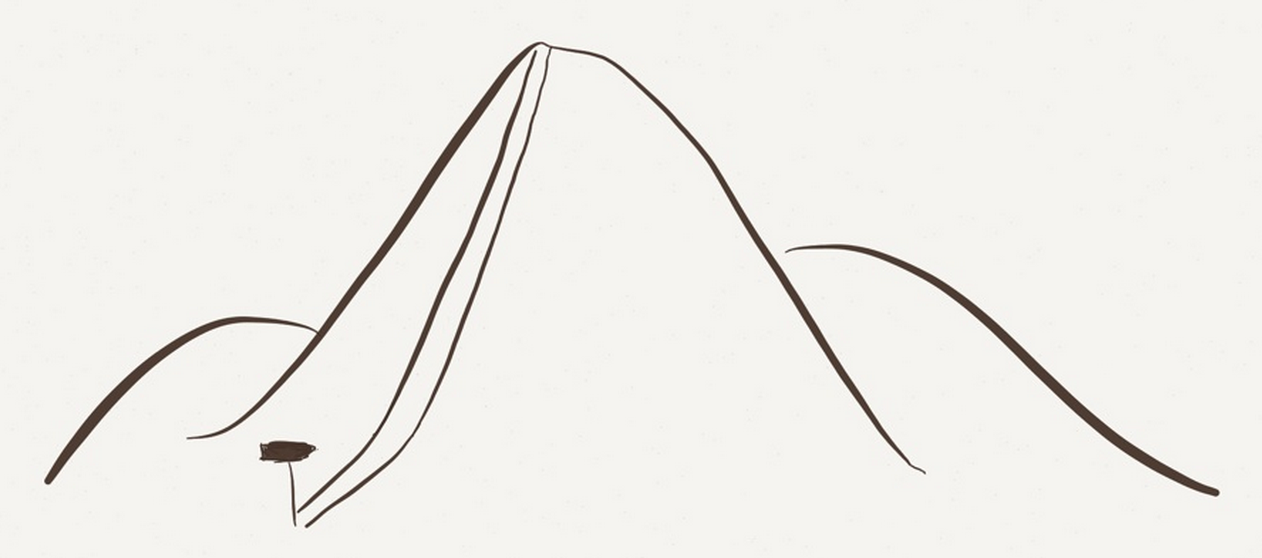
\includegraphics[width=0.28 \textwidth]{assets/final/straightMountain}
    }
\vspace{-20pt}
  \caption{Straight Learning Path}
  \label{fig:straight}
\vspace{5pt}  
      \fbox{
    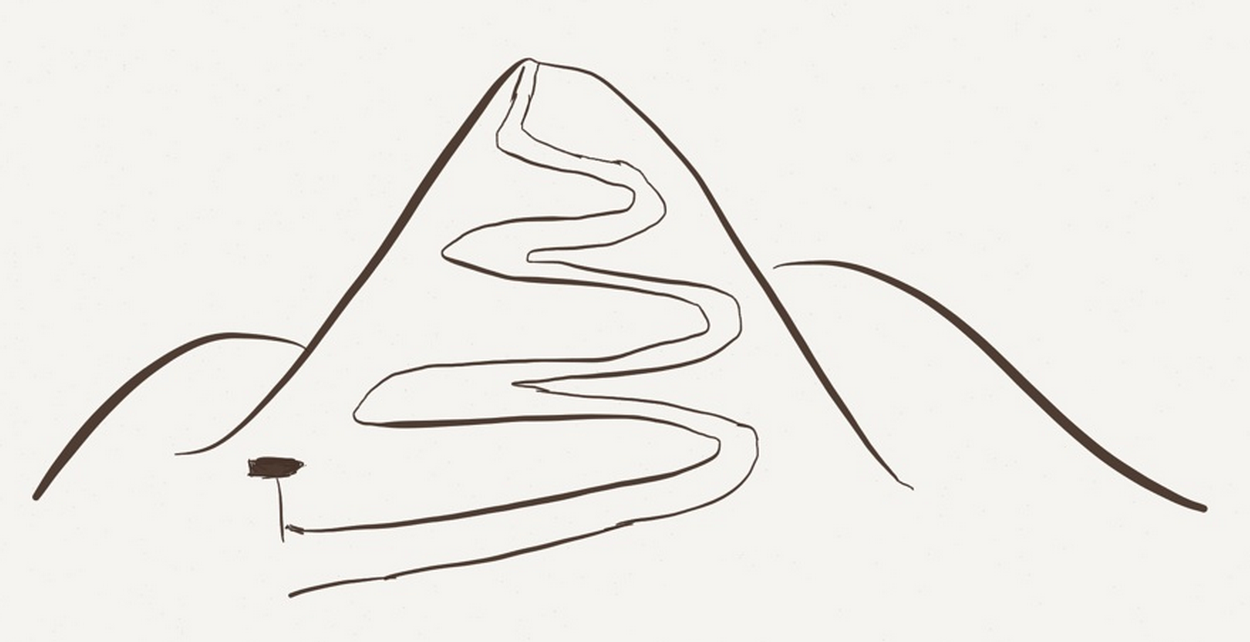
\includegraphics[width=0.28 \textwidth]{assets/final/curvyMountain}
    }

  \end{center}
\vspace{-20pt}
  \caption{Curvy Learning Path}
  \label{fig:curvy}
\vspace{-10pt}
\end{wrapfigure}

Learning new things is a bit like hiking up a mountain. If you have ever gone hiking, you know that it is relatively hard to hike up a steep mountain directly as shown in \autoref{fig:straight}. Some people do it but most people will rather hike up as shown in \autoref{fig:curvy}. Both paths lead to the goal. Within education, there is normally only one straight path. That is true for the narration in books, movies, and also traditional slide-based presentations. This has not changed in decades. With the advancement of technology, we are however able to change the way presentations and their narratives work. We can make it possible to link content that logically belongs together, in other words, content that is semantically close. Through the linking of content it can become possible for a presenter to seamlessly lead an audience, not along a predetermined straight path, but rather along the path that will allow the audience to take small detours and ultimately make the most out of the presentation.\\

This idea of linking content is not new. When Tim Berners-Lee laid out his Semantic Web Roadmap \cite{BernersLee:tsw98}, its intention was to transform the World Wide Web (WWW) from a web of mere human readable information to an information web with relations between different resources. Both the semantic web and the research at hand strive to connect pieces of information through adding context and thus to not just provide information, but rather knowledge. Within presentations, the intention is to present information in an interconnected way that provides context and thus facilitates understanding and learning.\\

\begin{wrapfigure}{l}{0.45\textwidth}
\vspace{-28pt}
  \begin{center}
  \fbox{
    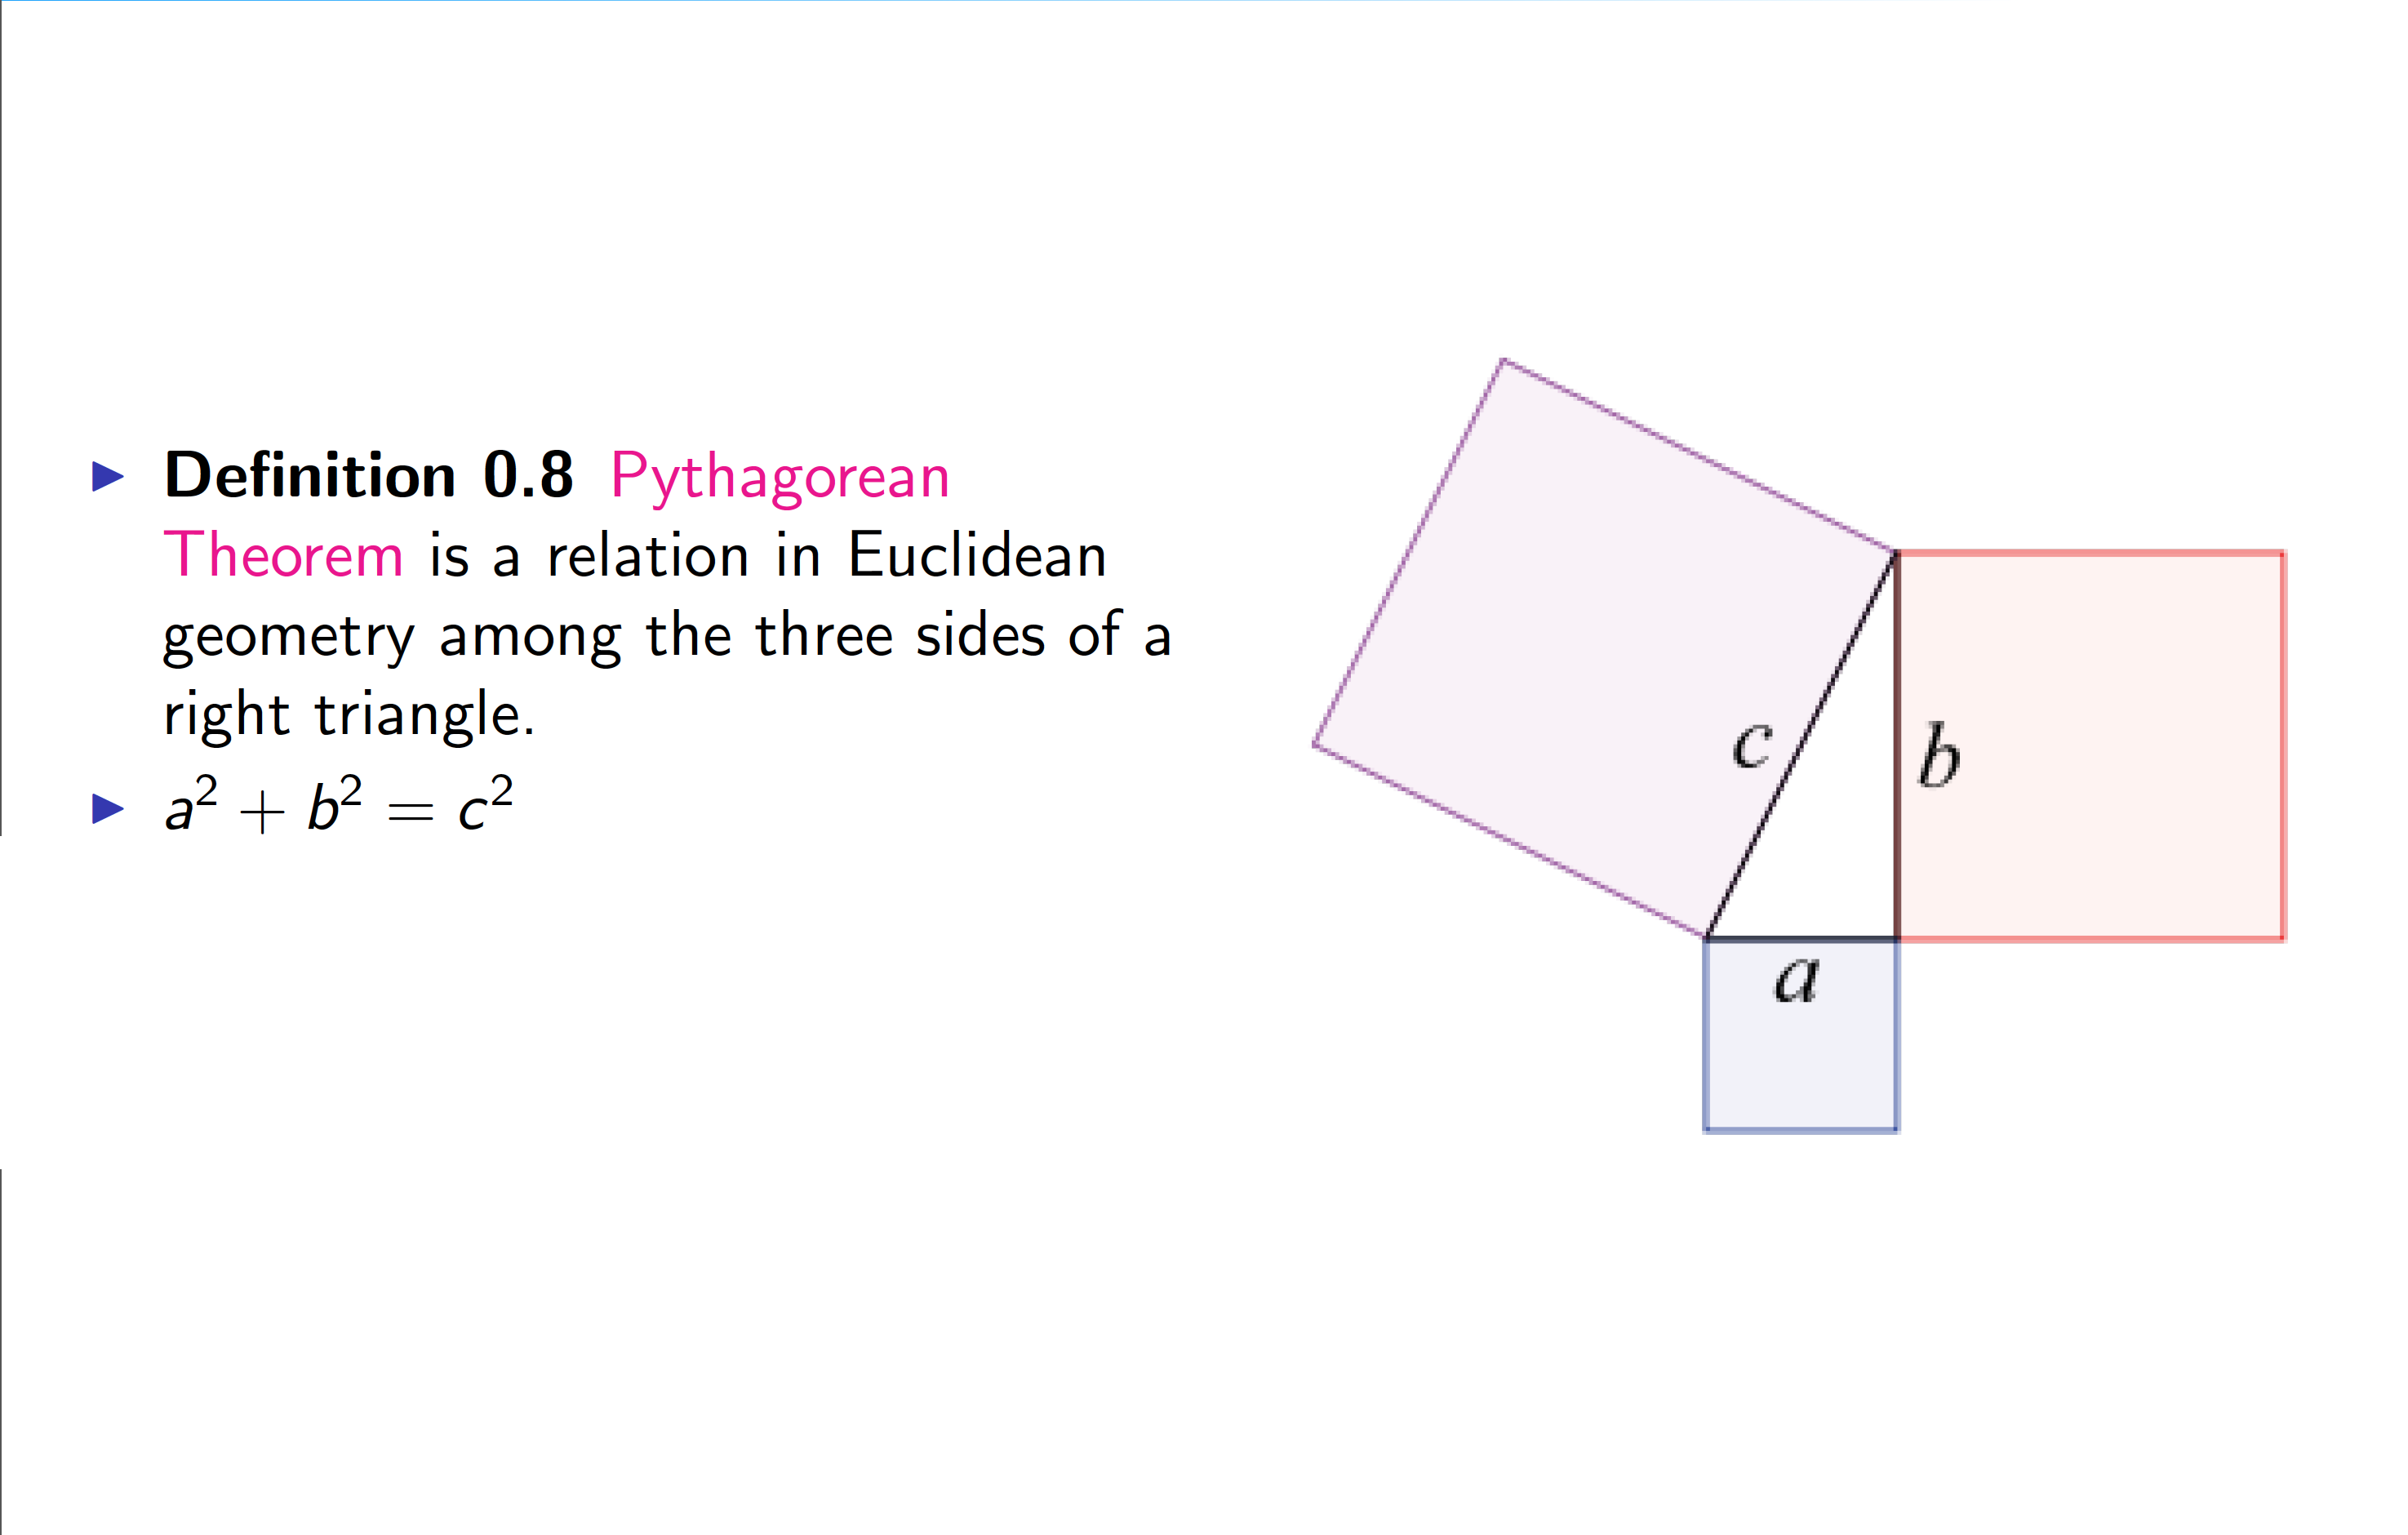
\includegraphics[width=0.43 \textwidth]{assets/final/slide_theorem}
    }
  \end{center}
\vspace{-20pt}
  \caption{Theorem Slide}
  \label{fig:slideP}
\vspace{-15pt}
\end{wrapfigure}

Let us dive into a contrived story that will guide us throughout this research: Annie, a young student learning mathematics, is watching her teacher give a presentation on how to use the Pythagorean theorem (see \autoref{fig:slideP}). She is then given a triangle with sides a = 3 cm and b = 4 cm. Now she wants to use the theorem to calculate the length of side c. Annie already knows how to calculate the square of a number and thus calculates that $c^2 = 25 \implies c = 5$. However Annie made a mistake and did not know what a right triangle is. Her teacher tells her that the question was a trick question and that the answer is wrong because the triangle she calculated this for is not a right triangle. Now Annie has to try to find out what a right triangle is.\\

\begin{wrapfigure}{r}{0.4\textwidth}
\vspace{-28pt}
  \begin{center}
  \fbox{
    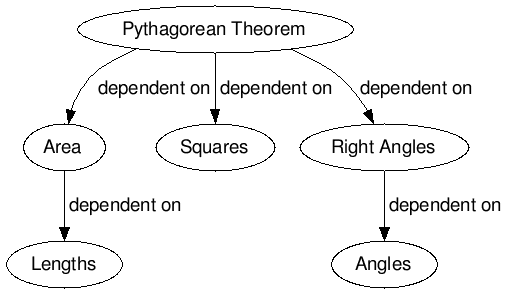
\includegraphics[width=0.38 \textwidth]{assets/final/PythDep}
    }
  \end{center}
\vspace{-20pt}
  \caption{Information Dependency of the Pythagorean Theorem}
  \label{fig:deppyg}
\vspace{-10pt}
\end{wrapfigure}

Annie's example shows the dependencies of different pieces of information (see \autoref{fig:deppyg}), i.e. the Pythagorean theorem depends on knowledge of area calculation, lengths, squares, right angles, and angles. As Annie and many of us who have witnessed many presentations know, traditional slide-based presentations lack the connectivity and flexibility to allow us to directly look related topics up. By adding connectivity and flexibility, we would allow Annie to not just look up the prerequisite knowledge such as what right angles are but hopefully also to understand the Pythagorean theorem.\\

To achieve our goal to help Annie, we will set out to create a relational presentation system \sys to visually present information and its context which allows Annie to interact with the content and choose a path that matches her knowledge base. For this we will be using the OMDoc (\textbf{O}pen \textbf{M}athematical \textbf{Doc}uments) format which, given an annotated set of documents, will provide us with the necessary XHTML-representation and PDF-representation of the information \cite{Kohlhase:OMDoc1.2}. It will also allow us to extract information about the semantic closeness of different pieces of information.\\

This information alone would tell Annie where she might find the information she seeks but it will only serve as a starting point. In face, this information will be used to visualize the dependencies of the information in a simple but effective approach using the presentation framework impress.js \cite{JSImpress:npentrel14}. The visualization of the information will make use of spatial narrative to connect information in a logical way. Thus the final product will allow Annie to intuitively interact with the presentation to find the information she needs.\\

Along the way of helping Annie, we will explore the question of how to create a flexible presentation which allows Annie to choose her own path to explore the context of a topic as needed by browsing through related resources seamlessly. To create this presentation a tool for automatic contextual visualization of information will be introduced. Through the usage of both spatial narrative and semantic closeness of information it will connect information logically. The end product will be a presentations which allow Annie to choose her own path by interacting with the presentation to seamlessly explore related topics and brush up on half-forgotten topics like right angles.\\

It is left to the reader to think about examples in his or her own life where he or she would have appreciated having this type of flexible presentations. There are many stories such as Annie's in real life and it is therefore important to provide this context to facilitate learning and knowledge transfer as a whole so that each of us can choose a learning path that allows us to reach the goal, whether it be by following a straight or a curvy path.

\section{Related Work}
\label{sec:relatedworks}

When searching for related work there is little to be found. Some works have focused on making teaching more effective by providing students with all lecture materials directly after class which has been found to have a positive influence on learning \cite{DBLP:dblp_journals/tochi/BrothertonA04}. For this purpose, systems that can automatically capture and index classroom events as videos and images have been devised \cite{indexedclass:npentrel14}. Some of these systems use temporal information \cite{DBLP:dblp_journals/isci/ChungS97} to show multiple resources in sync as they appeared in the lecture. However, while this approach also aims at improving the learning experience, it does not in any way link content semantically based on dependencies or allow for more interactive presentations through combining semantic closeness and spatial narrative.\\

Another piece of research has focused on the automatic generation of mind maps from text \cite{abdeen2009direct}. The software they developed uses Semantic Web technologies to create mind maps that show the relations between nodes that represent different objects. While the research at hand also intends to show the relation between pieces of information, it does it on a different level. For instance, it can represent that Shakespeare lived in Stratford but it would not be able to show the dependencies of mathematical concepts as it is limited to representing nodes in single words within the mind map. This research, on the other hand, will focus on exactly that, i.e. dependencies and the creation of interactive presentations.\\

There has also been research focusing on guided tours in mathematics \cite{SieBen:acgap00}. This creates guided tours on topics depending on the background of the user. While working towards the same goal, namely to improve knowledge transfer, it differs from this work in its presentation format. While Siekmann et al., focused on one topic and displaying it differently to users with different backgrounds, this research will show the topics of a whole course while allowing to see dependencies and while allowing to diverge from the prescribed presentation path.\\

Adding on to the research about guided tours in mathematics, there has also been research on semantic document navigation \cite{Koh:NavigationInMathDocs2012}. It demonstrates the need for assistance in form of navigation support for the reading of mathematical documents by creating a system that allows for semantic navigation in Excel spreadsheets. This research underlines the importance of a system that allows users like Annie to navigate information according to dependencies.
  
\section{Preliminaries}
\label{sec:preliminaries}

In the following we will examine some prerequisite knowledge. By engaging with our example presentation we will show how the presentation can be improved to transfer knowledge more effectively.

\subsection{Terminology}
\label{sec:terminology}

Before discussing the buzzword knowledge transfer further, we will first engage in the conceptualization of the terms \textit{information}, \textit{knowledge}, and \textit{context}.\\

The Oxford Dictionary of English \cite{OED:npentrel14} defines \textit{information} as "what is conveyed or represented by a particular arrangement or sequence of things". Recalling \autoref{fig:slideP} and our contrived story of Annie, an example for information is the sequence \textit{$a^2 + b^2 = c^2$}. For the term \textit{knowledge}, we will use the definition in Merriam-Webster's thesaurus \cite{Webster:npentrel14} which defines it as the "fact or condition of knowing something with familiarity gained through experience or association". This \textit{association} is of special importance for the current project. We will define it as knowledge that is made up out of several pieces of information that are connected. In the example from above knowledge would be knowing when and how the Pythagorean theorem can be used by knowing the information that the usage of the Pythagorean theorem depends on (see \autoref{fig:deppyg} above).\\ 

According to the Merriam-Webster thesaurus \cite{Webster:npentrel14}, \textit{context} is defined as "the parts of a discourse that surround a word or passage and can throw light on its meaning". Context can be easily explained with the example of Annie learning the Pythagorean theorem. The \textit{information} about the calculation of the length of the third side of the triangle is only helpful for Annie within the \textit{context} of the pieces of \textit{information} this depends on. Without this \textit{context}, Annie cannot understand the theorem. Figure \ref{fig:deppyg} above illustrates the context by showing the dependencies of the theorem, i.e. calculating squares, area calculation, triangles, and right angles. It represents relatedness of \textit{concepts} by linking the different \textit{concepts} with lines, thus creating \textit{associations} between the different pieces of \textit{information}. The relatedness between the relevant concepts can also be imagined as a network. We will be using the terms \textit{context} and \textit{network} almost interchangeably and depend on the reader to have the right intuition about these terms.

\subsection{OMDoc}
\label{sec:OMDoc}

OMDoc \cite{Kohlhase:OMDoc1.2} is an XML-based system that provides a data model and a format for content markup for mathematical documents. As such it is a semi-formal domain ontology. An ontology provides the framework for creating a semantic structure. It formally describes concepts within a specified area. A semi-formal ontology \cite{Sheth:npentrel14} is an ontology where formality of semantics is not a given. The semi-formal ontology can consist of partial or incomplete knowledge. \\

If OMDoc was used in every part of mathematics (and related fields), we would have a repository of mathematical knowledge that could be processed in various ways. This is possible because OMDoc provides the framework to create and store mathematical objects such as definitions and concepts. The relations between different mathematical objects and the attributes of mathematical objects can be added through annotations. This elevates the net of separate pieces of information that are stored individually to a semantic representation and can be used to improve knowledge transfer.


\subsection{Status of Information within the (Dis)Course}
\label{sec:infostatus}

In linguistics the concept of information packaging \cite{CambridgeGrammar:npentrel14} is well known and widely discussed. Within the study of \textit{information structure}, one discriminates between \textit{familiar/ old} and \textit{unfamiliar/ new} information. \textit{Familiar/ old} information is shared by speaker and addressee, i.e. it is in the intersection of knowledge of student and teacher. \textit{New/ unfamiliar} information is not in the shared knowledge base or the content commons \cite{CNX:whitepaper}. In addition, one distinguishes information that is old or new with respect to the discourse or with respect to the addressee.

\begin{center}
\textit{"My sister went to the circus the other day; \underline{she} said \underline{it} was brilliant."}\\
\end{center}

In this example in the first part of the sentence, \textit{discourse-new} information pertaining to my sister and to a circus is introduced. In the second part, the underlined parts are considered \textit{discourse-old} since they have already been introduced. These terms are coined to refer to the accessibility of the information to participants of the discourse \cite{Newness:npentrel14}. The accessibility depends on the relative \textit{newness}, i.e. recency of mention, of this information.\\

These concepts can be adapted to the situation of teaching mathematics or computer science to students in a class. In general we will call the information that the speaker is passing on to the addressees/students \textit{course-new}. Since we are in the setting of a university course, the \textit{course-new} information will generally depend on information that is \textit{course-old}. We will additionally introduce a third modus for information called \textit{course-ancient}. This covers the situation where the addressee has difficulties following the speaker since the \textit{course-new} information depends on \textit{course-old} information that might be 'too old' to be easily remembered, i.e. \textit{course-ancient}.\\

Going back to the example of Annie, the information about the Pythagorean theorem that the teacher is just introducing would be considered \textit{course-new}. The information about the right angle which Annie cannot access anymore since she was taught about this too long ago is \textit{course-ancient}. The information about squares which Annie still remembers is \textit{course-old}. Through the semantic closeness that OMDoc provides, we will be able to determine the status of information within the (dis)course.

\subsection{Primitives}
\label{sec:primitives}

Within knowledge representation, five evaluation criteria for knowledge representation are known \cite{Kohlhase:Complog:base}: Expressive Adequacy, Reasoning Efficiency, Primitives, Meta-representation, and Incompleteness. Primitives are the different elements of representation. In terms of evaluation it is important to have intuitive primitive elements. The primitive elements can be further subdivided into structural and semantic primitives \cite{DBLP:dblp_conf/acl/Salveter80}. The structural primitives have little inherent semantics associated with them whereas the semantic primitives carry meaning.\\

Visual and normal tree-like graph language have different primitives and it is interesting how the primitives of the former can be mapped to the primitives of the latter. When we consider tree-like graphs, there are two structural primitives, namely the nodes, which represent concepts, and the edges, which represent relations between nodes. Additionally we can add semantic primitives like attributes to the concepts and to the relations to add information or to show what kind of a relation it is. In normal graphs a relation between two nodes is often quite simple: there is one node that acts as the subject, one node that acts as an object, and the relation that acts as a predicate. Thus we can, for instance, express that the Pythagorean theorem depends on information about right angles (similar to \autoref{fig:deppyg}). These structural primitives and semantic primitives provide the basics that information graphs can be built on.\\

For impress.js, the primitive elements are text, images, slides, and the visual relation between the different slide-like structures. The slides can be mapped directly to the nodes/concepts which graphs use. Text and images are taken for granted within the slides. Similarly, the visual relation between different slides is very much like the relations between nodes. However, the relations can be much more expressive within impress.js.\\

These relations or connections between different slides do not just connect content that depends on one another but also content that has a temporal connection, similar to slides following one after another. As such the temporal associations show the path that a traditional lecture would take. The dependencies that are visualized around each slide, mainly above or below the slide, allow for additional interactivity.

\subsection{Spatial Narrative}
\label{sec:spatialnarrative}

The development of presentation tools like impress.js and Prezi, has changed how people think about presentations while making use of spatial narrative. Prezi is "a virtual whiteboard that transforms presentations from monologues into conversations: enabling people to see, understand, and remember ideas" \cite{Prezi:npentrel14}. When doing a good prezi presentation one has to understand the topic one is presenting on a deeper level and think about how one can portray connections between content visually.\\

The concept of Spatial Narrative stems from the establishment of frameworks for "the creation of computer-assisted flexible \textit{guided tours} based on the thematically and narrative linking of a set of locations within an area into a \textit{spatial narrative}" \cite{SpatialNarratives:npentrel14}. Teachers that are presenting a topic are an example for the experience of a tour guide for a certain topic.\\

The benefit of spatial narrative is that the audience gains a more thorough understanding of the subject and has a better understanding of the interconnections between different pieces of information. By providing the audience with a story as a narrative one also makes use of the concept of Storytelling which is largely accredited with the benefit that the audience will have an easier time following the presenter. That is the case because our brains are not made to memorize a lot of unconnected pieces of information; it is far easier for us to remember information if it comes in story form \cite{Storytelling:npentrel14}.\\

\begin{wrapfigure}{r}{0.45\textwidth}
\vspace{-28pt}
  \begin{center}
  \fbox{
    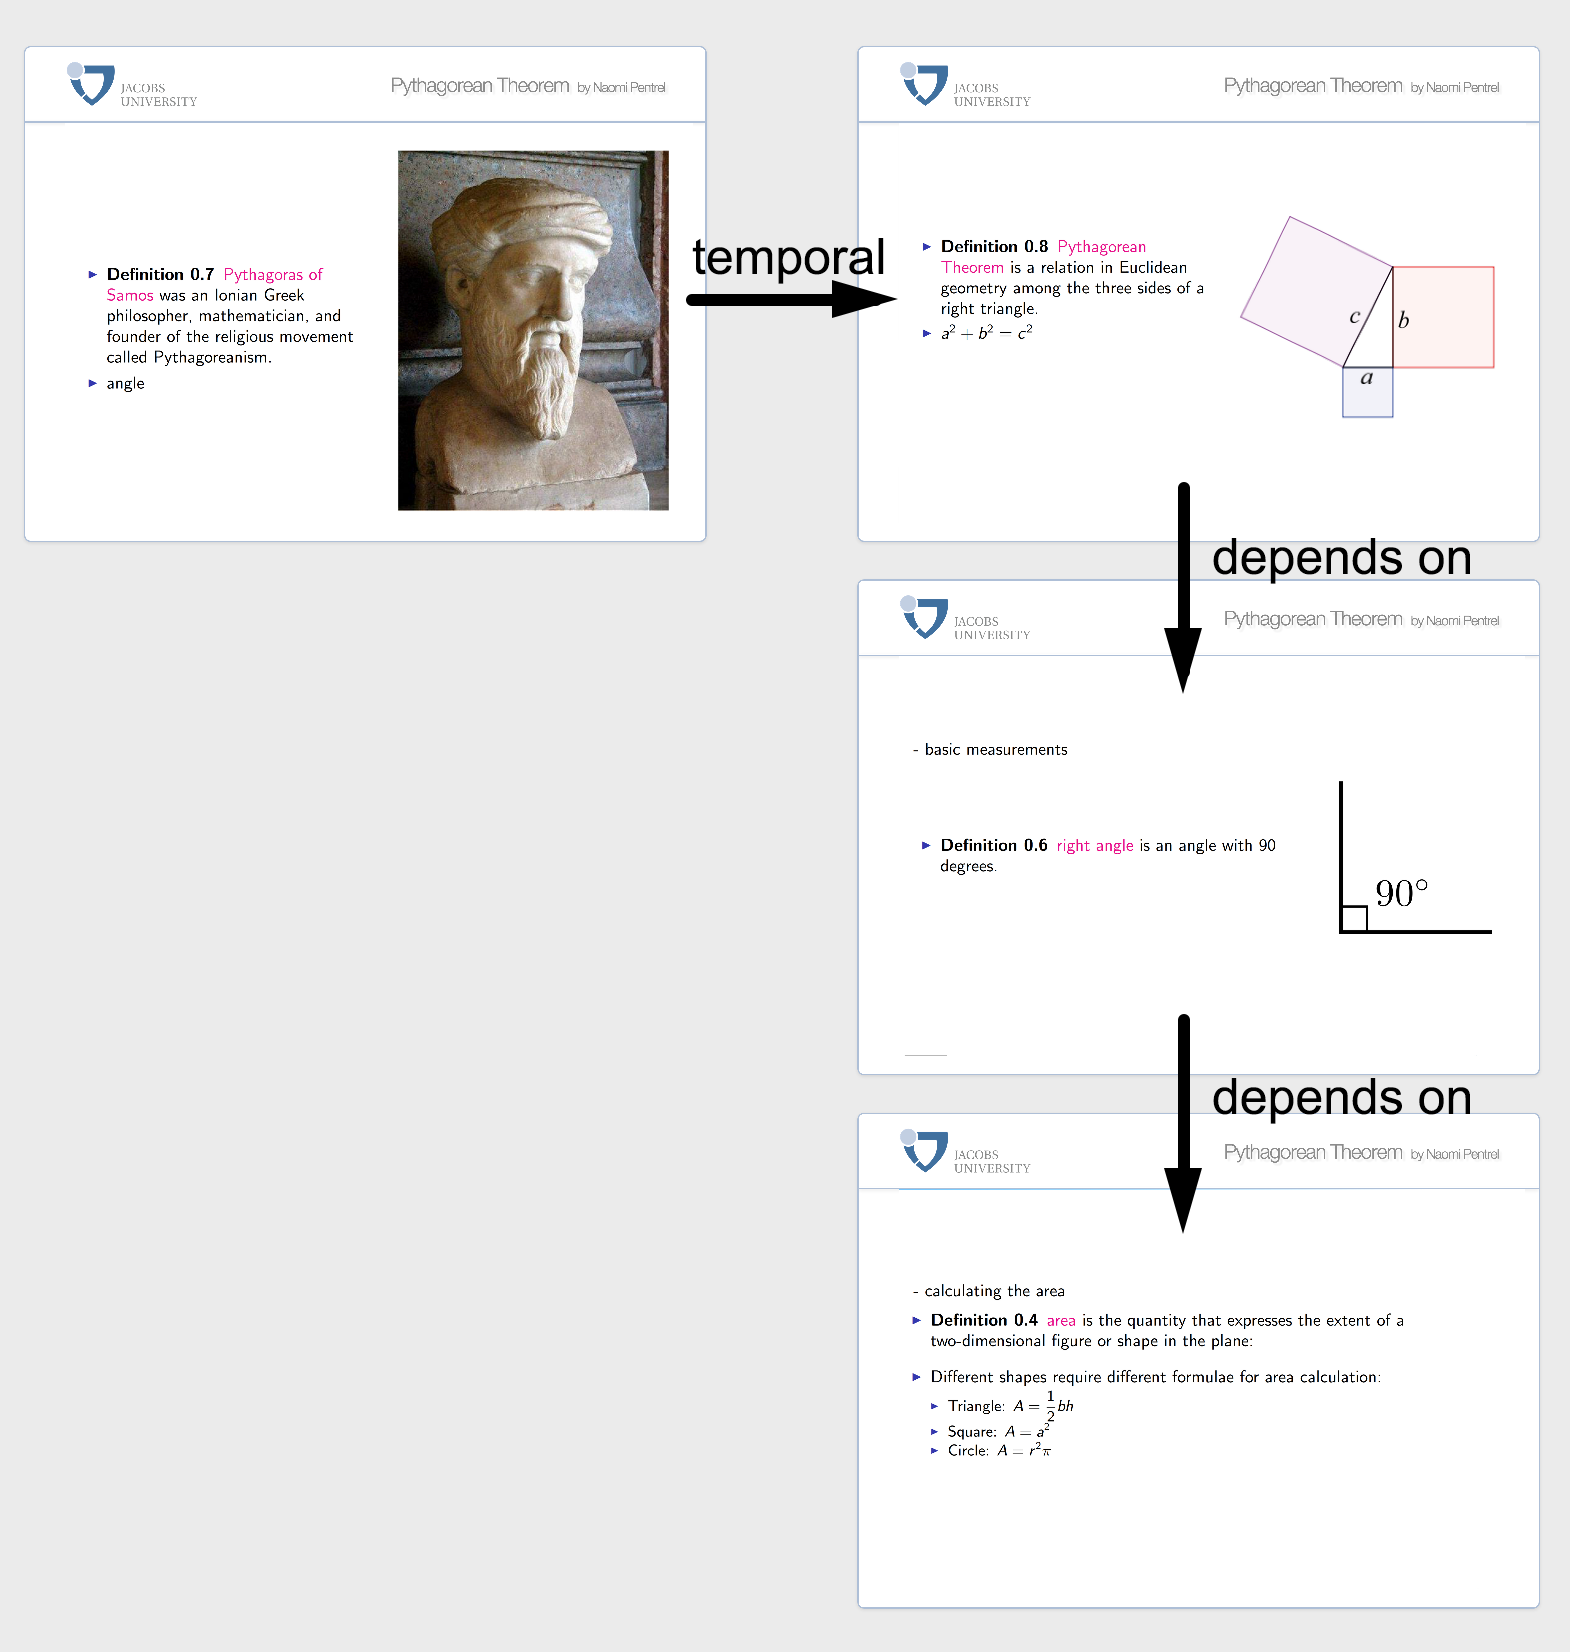
\includegraphics[width=0.43 \textwidth]{assets/final/arrowsPyth}
    }
  \end{center}
\vspace{-20pt}
  \caption{Connection of Slide}
  \label{fig:arrowspyg}
\vspace{-10pt}
\end{wrapfigure}

In this research we will use this knowledge to form an interconnected network of information that tells a visual story based on semantic closeness to facilitate the transfer of knowledge. For Annie this means that she will be presented with the \textit{course-new} information about the Pythagorean theorem in a way that the dependent \textit{course-ancient} and \textit{course-old} information would be visually close and visually connected (see figure \ref{fig:arrowspyg}). It also means that Annie's teacher can answer Annie's questions easily by just going to the related \textit{course-ancient} information in an instant.

\subsection{impress.js}
\label{sec:Impressjs}

For the implementation of \sys, impress.js will be used, as commercial applications like Prezi, while more mature in presentations for the general crowd, do not provide us with an Application Programming Interface (API) that allows the generation of whole presentations. The open-source presentation framework \textbf{impress.js} \cite{JSImpress:npentrel14} was created by Bartek Szopka. It combines HTML and CSS3 which makes it highly customizable but unfortunately renders it unsupported by older browsers. The presentation data is entered in the HTML file; each slide in its own div with \texttt{data-x}, \texttt{data-y}, and \texttt{data-z} attributes to change the position of the slide. The \texttt{data-x} and \texttt{data-y} attributes change the position of the element according to the normal x- and y-axes. The \texttt{data-z} attribute changes the closeness of the elements along the z-axis.\\
\definecolor{bg}{rgb}{0.90,0.90,0.90}

\begin{wrapfigure}{r}{\textwidth}
\vspace{-26pt}
\begin{minted}[linenos=true, bgcolor=bg]{C}
<div class="step" data-x="1000" data-y="0">
  Slide Content
</div>
\end{minted}
\vspace{-8pt}
  \caption{Code Snippet to Create a Slide}
  \label{fig:SSlide}
  \vspace{12pt}
\end{wrapfigure}

\begin{wrapfigure}{r}{0.3\textwidth}
\vspace{-26pt}
  \begin{center}
  \fbox{
    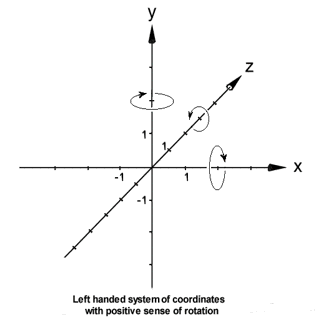
\includegraphics[width=0.28 \textwidth]{assets/rotate}
    }
  \end{center}
\vspace{-20pt}
  \caption{Rotations \cite{Rotations:npentrel14}}
  \label{fig:Rotate}
\vspace{-10pt}
\end{wrapfigure}

Apart from these basic attributes, impress.js offers the \texttt{data-scale} attribute to scale content, making slides appear bigger or smaller, and the \texttt{data-rotate} attribute which rotates slides in 3 dimensions using \texttt{data-rotate-x}, \texttt{data-rotate-y}, and \texttt{data-rotate-z}. As shown in \autoref{fig:Rotate} this allows the presentation to go into the third dimension.\\

In the following code snippets, a few other basic functionalities are illustrated \cite{andismith:npentrel15}. The opacity attribute allows us to discriminate between active and inactive slides which allows us to hide content so as not show too much information to a user at once. Adding an overview can be accomplished with the last part of the CSS snippet and the HTML snippet below that.

\begin{wrapfigure}{l}{\textwidth}
\vspace{0pt}
\begin{minted}[linenos=true, bgcolor=bg]{C}
.step { opacity: 0.2; }
.step.active { opacity: 1; }
.step-overview .step { opacity: 1; cursor: pointer; }
\end{minted}
\vspace{-8pt}
  \caption{Code Snippet to Show and Hide Content}
  \label{fig:SSlide}
  \vspace{20pt}
\end{wrapfigure}

\begin{wrapfigure}{l}{\textwidth}
\vspace{-10pt}
\begin{minted}[linenos=true, bgcolor=bg]{C}
<div id="overview" class="step" data-x="8000" data-y="1000" data-scale="10">
</div>
\end{minted}
\vspace{-11pt}
  \caption{Code Snippet for an Overview}
  \label{fig:SSlide}
  \vspace{12pt}
\end{wrapfigure}

\begin{wrapfigure}{l}{\textwidth}
\vspace{-50pt}
\end{wrapfigure}

To link back to a slide, slides are accessible via IDs. The slide with the ID \texttt{conclusion} will thus be accessible by appending \texttt{\#/conclusion} to the end of the URL.

\section{Towards a More Effective Presentation Format}
\label{sec:TowardsAMoreEffectivePresentationFormat}

Building on the preliminaries, we will now commence the journey towards building a more effective presentation format to improve knowledge transfer by allowing flexibility in presentations. To create these presentations automatically, the tool \sys \cite{npentrel:npentrel15} was created.\\

\begin{wrapfigure}{l}{\textwidth}
\vspace{-0pt}
  \begin{center}
  \fbox{
      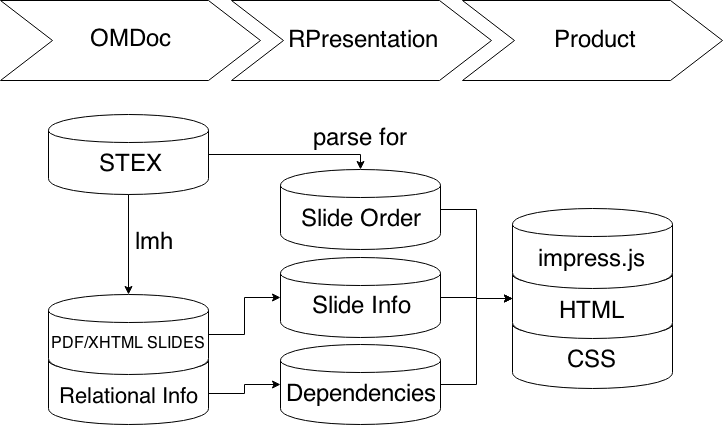
\includegraphics[width=0.70\textwidth]{assets/final/Architecture}
    } 
\vspace{-6pt}
  \caption{Architecture Diagram}
  \label{fig:architecture}
\vspace{12pt}
  \end{center}
\end{wrapfigure}

\begin{wrapfigure}{l}{\textwidth}
\vspace{-50pt}
\end{wrapfigure}

With the OMDoc framework and its tools it is possible to write down course notes or other documents in \textbf{S}emantically enhanced \TeX / \LaTeX\ (\stex). The Local MathHub Tool (lmh) uses these to create, among other things, PDF slides, XHTML slides, and relational information. To help Annie, let us use a document that explains the Pythagorean theorem and related topics. The files that lmh creates, along with the \stex -files will be used as input in the next steps. For the implementation of  \sys Java was used. It would have been possible to choose other programming languages, however, using Java, we end up with platform-independent code.\\

\sys itself operates in five main steps:\\
\vspace{-12pt}
\begin{enumerate}[topsep=0pt,itemsep=-1ex,partopsep=1ex,parsep=1ex]
\item Get user input for the locations and names of folders.
\item Parse \sTeX to retrieve the order of slides.
\item Extract dependencies from relational info.
\item Extract necessary XHTML or PNG parts for slides.
\item Create presentation.
\end{enumerate}
\vspace{5pt}

After asking the user for the location and names of the folders we want to work on, \sys can parse the provided \stex files in a recursive fashion to retrieve the slide order. It does this by starting with a given top level file which includes other files via \textit{mhinputref}s.\\

In the next step the relational information is parsed and put into a hashtable. The keys are the slides which link to an array of dependent slides. The order of the slides and their dependencies are then combined to an information graph which we use to create a relational presentation out of the annotated document using the slide info. This slide information is created by either parsing the XHTML and directly copying the needed parts into the final presentation or by transforming the PDF into PNGs that are then included in the final presentation.\\

For including the XHTML or the PNGs we use self-created boilerplate code, in which only some coordinates and the XHTML or the PNGs for the slide are added (see \autoref{sec:Impressjs}). The details of this process will be explained in subsection \ref{sec:narrativePaths}, \ref{sec:orderedInfoGraphs}, and \ref{sec:levels}. To complement the HTML, a CSS stylesheet is added which adds the some design elements. The design of the template is based on a presentation by S. Wolf \cite{Wolf:npentrel15}.\\

To bring the presentation to life the library impress.js which was introduced in \autoref{sec:Impressjs} is used because it makes it simple to reuse the XHTML code that was automatically generated by lmh. An important additional reason for the choice of impress.js \cite{JSImpress:npentrel14} is that it enables us to use spatial Narrative as discussed in \autoref{sec:spatialnarrative} and \autoref{sec:Impressjs}. The library impress.js works in all modern browsers that support CSS 3D transforms; some older and mobile browsers are, however, not able to display the created presentations properly.

\subsection{Narrative Paths}
\label{sec:narrativePaths}

The information that OMDoc provides us with could also be simply visualized as a tree of information. But this would not be very engaging and it would be hard for a person to process. Similarly, traditional slide-based presentations do not provide a very engaging or interactive form of presenting information. Therefore we will focus on using spatial narrative to make presentations more engaging and enhance knowledge transfer.\\ 

One opportunity to employ spatial narrative is to place content which is inherently related visually close together since this conveys the meaning that these objects belong together. In \textit{A mathematical approach to ontology authoring and documentation} \cite{LK:MathOntoAuthDoc09}, it is stated that "documents consist of narrative and content layers". In our case, the content layers are the mathematical objects, i.e. the statements or theories. Narrative layers refer to the order in which the mathematical objects from content layers are presented.\\

\begin{wrapfigure}{c}{\textwidth}
\vspace{-0pt}
  \begin{center}
  \fbox{
      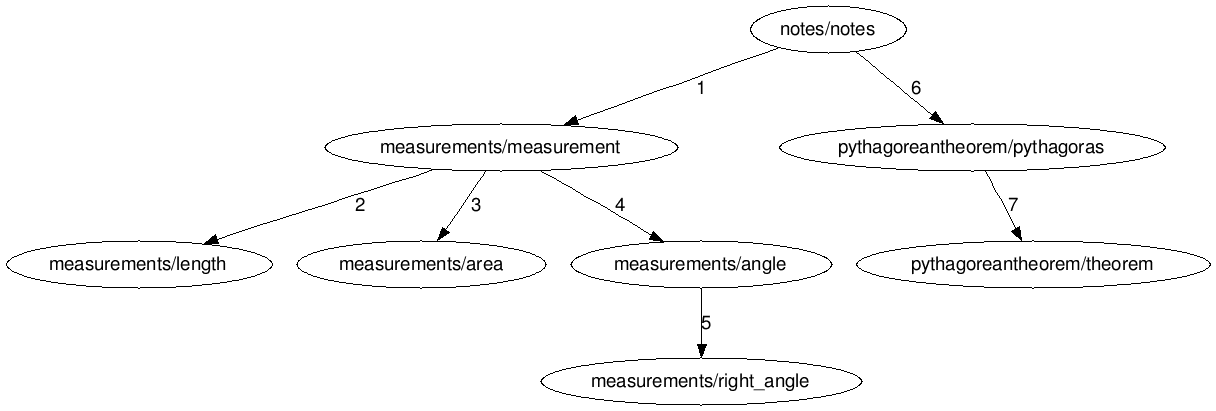
\includegraphics[width=0.87\textwidth]{assets/final/inclusionGraphPythagorean}
    } 
\vspace{-8pt}
  \caption{Inclusion Graph for the Pythagorean Theorem}
  \label{fig:inclusionGraph}
\vspace{12pt}
  \end{center}
\end{wrapfigure}

\begin{wrapfigure}{l}{0.3\textwidth}
\vspace{-28pt}
  \begin{center}
  \fbox{
      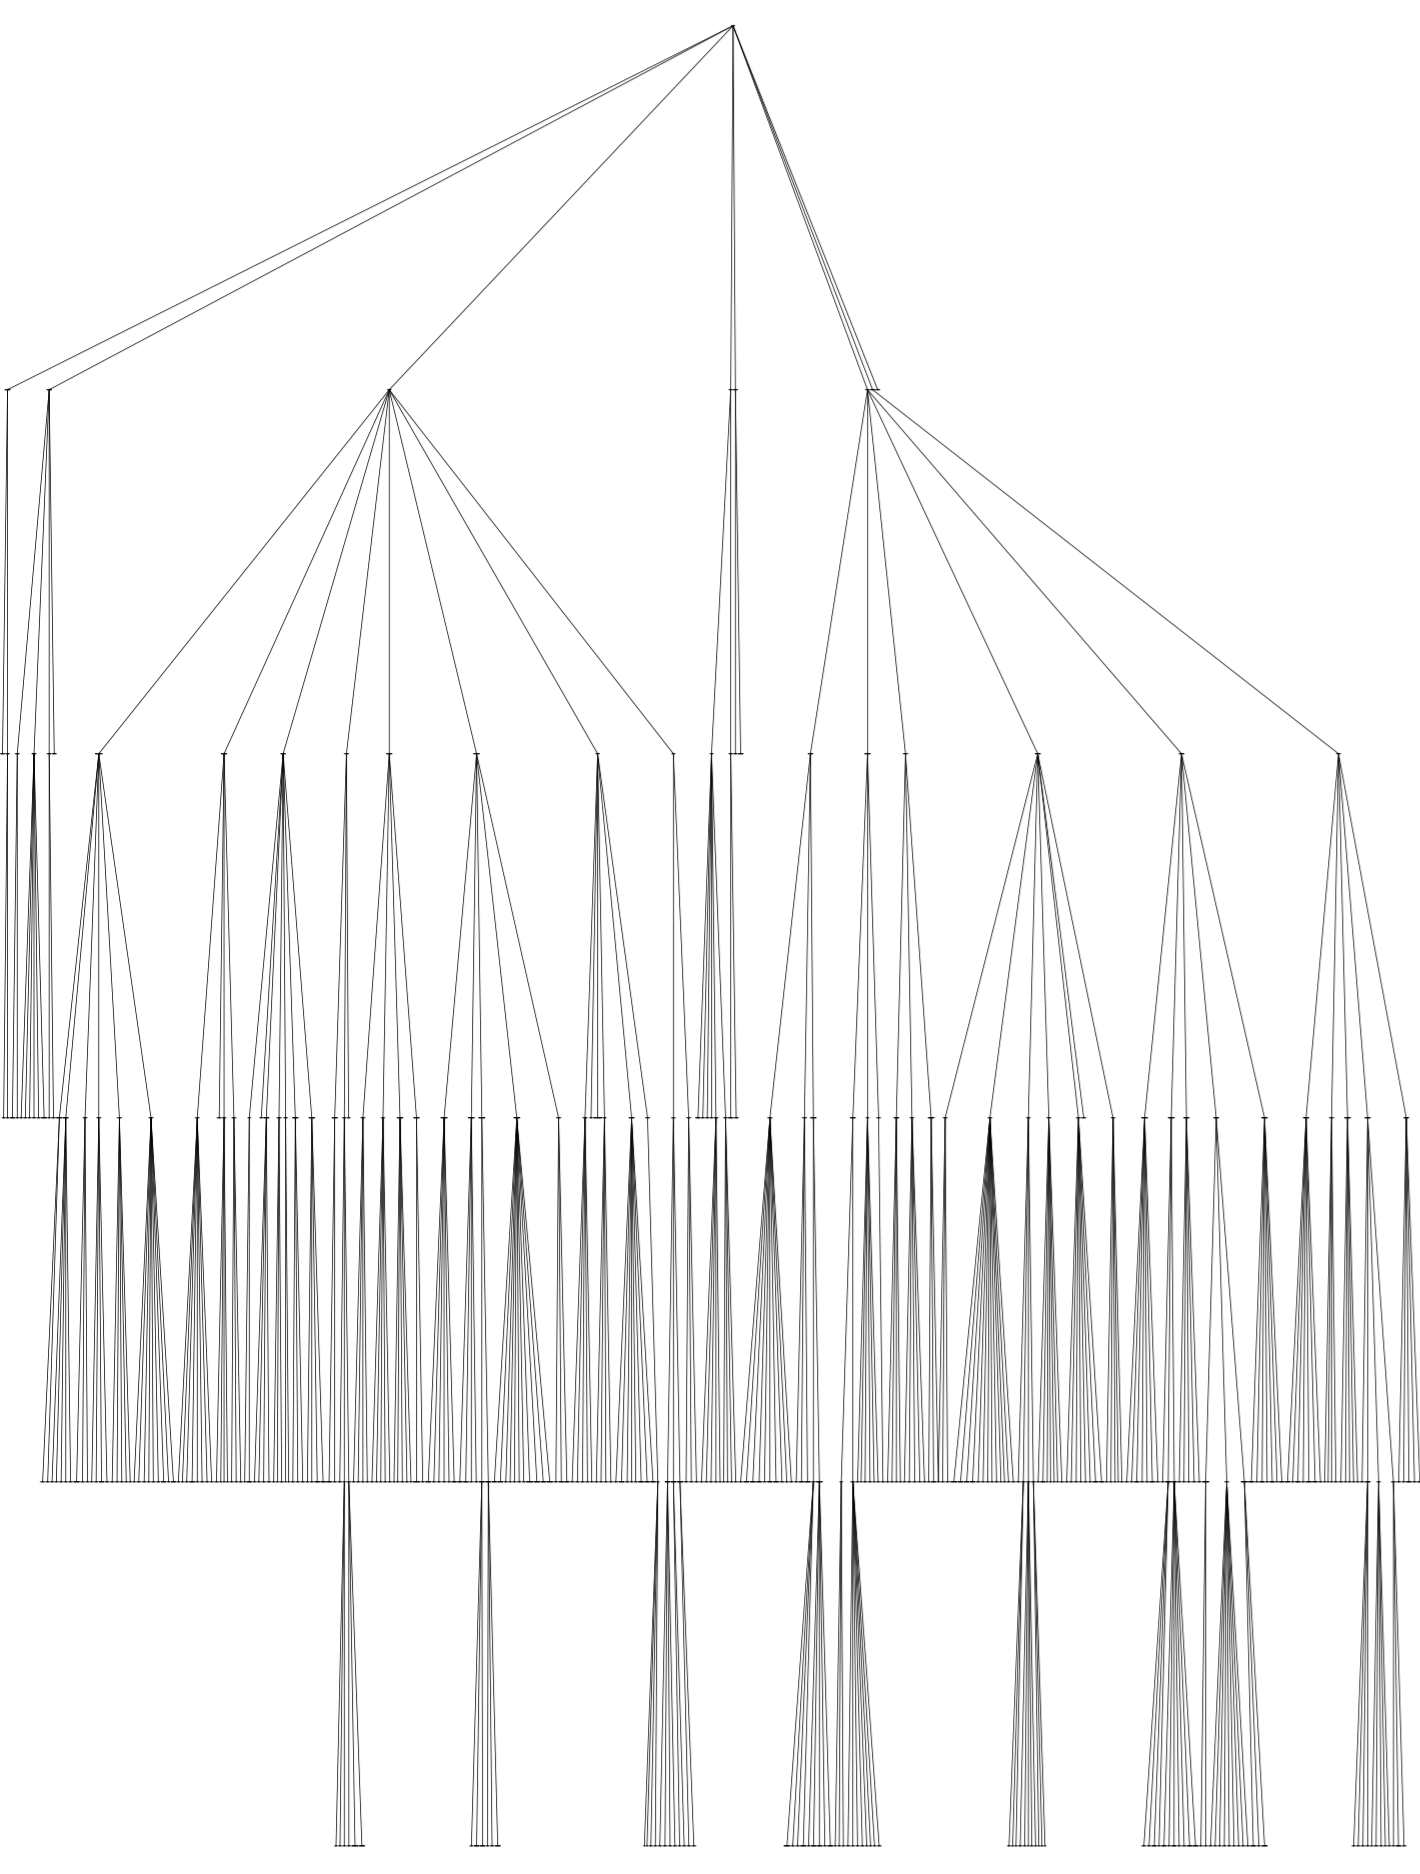
\includegraphics[width=0.28\textwidth]{assets/final/inclusionGraphCS}
    } 
\vspace{-20pt}
  \caption{Inclusion Graph for GenCS}
  \label{fig:inclusionGraphGenCS}
\vspace{-24pt}
  \end{center}
\end{wrapfigure}

In our system, the \stex files are parsed using a Depth First Search algorithm to retrieve the narrative the writer intended to use. For the explanation of the Pythagorean theorem this can be seen in \autoref{fig:inclusionGraph}. The graph for a whole course like the General Computer Science course (GenCS) at Jacobs University Bremen \cite{Kohlhase:GenCSII:base} is too big to be shown properly (see \autoref{fig:inclusionGraphGenCS}).\\

The retrieved order is the intended narrative layer, which we will refer to as a \textit{primary narrative path} since we go from slide to slide on our path to the end of the presentation. To create this primary narrative path we need to add several slides with increasing x-coordinates as shown in \autoref{fig:narrativePathCode}. This code then creates the narrative path portrayed in \autoref{fig:primaryNarrativePath}.\\

\begin{wrapfigure}{r}{\textwidth}
\vspace{-20pt}
\begin{minted}[linenos=true, bgcolor=bg]{C}
<div class="step" data-x="1250" data-y="0"> ... </div>
<div class="step" data-x="2500" data-y="0"> ... </div>
\end{minted}
\vspace{-8pt}
  \caption{Code Snippet for a Narrative Path}
  \label{fig:narrativePathCode}
  \vspace{12pt}
\end{wrapfigure}

\begin{wrapfigure}{c}{\textwidth}
\vspace{-30pt}
  \begin{center}
  \fbox{
    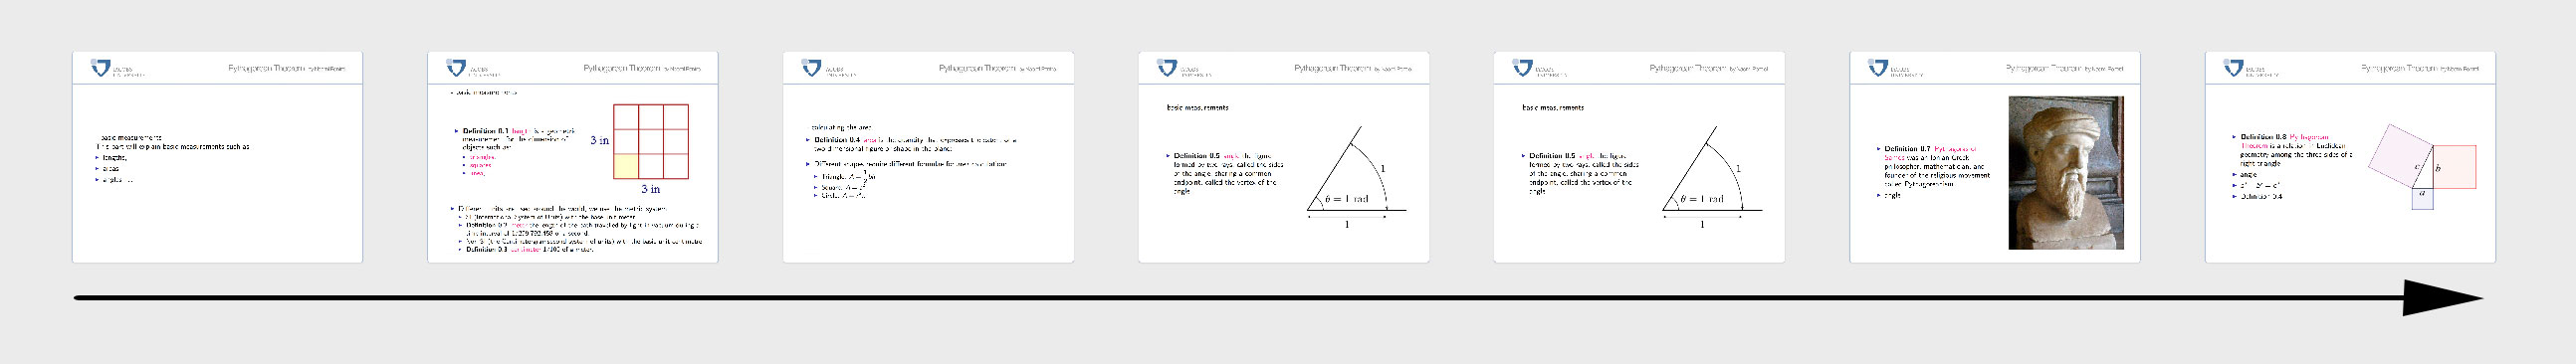
\includegraphics[width=0.97\textwidth]{assets/final/primaryNarrativePath2}
    }
  \end{center}
\vspace{-20pt}
  \caption{Primary Narrative Path}
  \label{fig:primaryNarrativePath}
\vspace{12pt}
\end{wrapfigure}

\begin{wrapfigure}{l}{\textwidth}
\vspace{-50pt}
\end{wrapfigure}

The primary narrative path, formed by a horizontal stream of slides, is the traditional path a presenter normally uses when preparing a PowerPoint presentation. This path happens to also contain temporal information which is illustrated by the arrow in \autoref{fig:primaryNarrativePath}. This temporal information is what we extracted from the \stex files as the order in which the slides (or the information on the slides) should appear.\\

This temporal information is also used to create narrative paths for subsections of the whole presentation that only explain one topic. These narrative paths are similar to the guided tours mentioned in \autoref{sec:relatedworks} in that they aim to explain one topic but they are different in that they just reuse slides that have already occurred. Going back to our example of Annie, an example of a subsection would be the information concerning angles. In essence, the \textit{intended narrative path} contains multiple \textit{narrative paths} of its own. These occur on different levels as explained in \autoref{sec:levels} and are based on the concept of spatial parratives (see \autoref{sec:spatialnarrative}).

\subsection{Ordered Information Graphs}
\label{sec:orderedInfoGraphs}

As described in \autoref{sec:TowardsAMoreEffectivePresentationFormat}, lmh outputs information about dependencies of topics. The general format of one relation can be seen in \autoref{fig:reldatacode} (lines 1-2). A specific example showing some of the dependencies for the Pythagorean theorem example can be seen in lines 4-11.\\

\begin{wrapfigure}{r}{\textwidth}
\vspace{-0pt}
\begin{minted}[linenos=true, bgcolor=bg]{C}
theory path/to/file?theory_name
Includes path/to/file path/to/dependent/file?theory_name

theory 
pythagoreantheorem/pythagoreantheorem/theorem.omdoc?pythagoreantheorem
Includes 
pythagoreantheorem/pythagoreantheorem/theorem.omdoc?pythagoreantheorem
pythagoreantheorem/measurements/right_angle.omdoc?right_angle
Includes 
pythagoreantheorem/pythagoreantheorem/theorem.omdoc?pythagoreantheorem
pythagoreantheorem/measurements/area.omdoc?area
\end{minted}
\vspace{-5pt}
  \caption[Caption for LOF]{Code Snippet of Relational Data \footnotemark}
  \label{fig:reldatacode}
  \vspace{12pt}
\end{wrapfigure}

\begin{wrapfigure}{l}{\textwidth}
\vspace{-50pt}
\end{wrapfigure}

\footnotetext{All the above paths were shortened by "http://mathhub.info/MiKoMH/" to maintain readability.}

The system \sys parses the relational data and thus retrieves the dependencies of the topics which are visualized for Annie's example in \autoref{fig:depGraphPythagoreanFull}. Dependencies give us the \textit{course-ancient} information, as dependencies intuitively link to information likely obtained longer ago.\\

\begin{wrapfigure}{c}{\textwidth}
\vspace{-30pt}
  \begin{center}
  \fbox{
      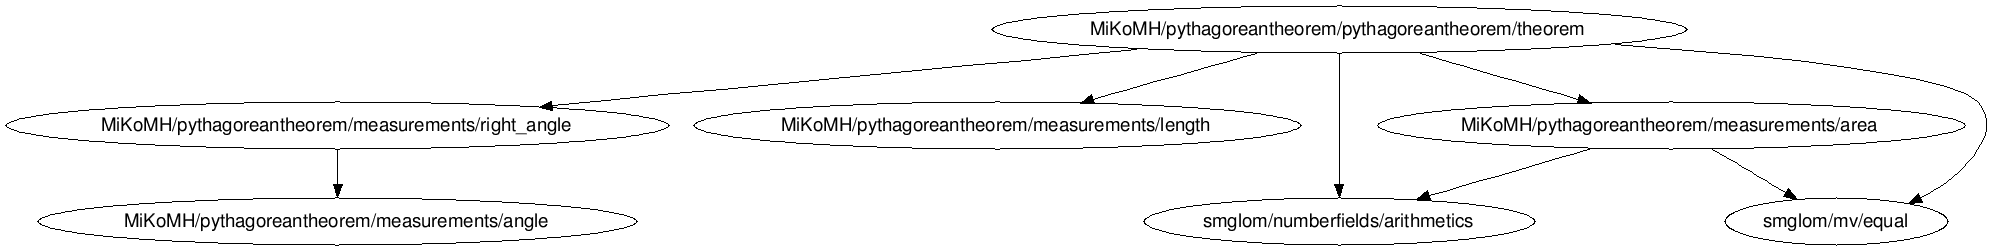
\includegraphics[width=0.97\textwidth]{assets/final/dependencyGraphPythTheo2}
    } 
\vspace{-20pt}
  \caption{Dependency Graph}
  \label{fig:depGraphPythagoreanFull}
\vspace{0pt}
  \end{center}
\end{wrapfigure}

\begin{wrapfigure}{c}{\textwidth}
\vspace{-60pt}
\end{wrapfigure}

With the data about the order and the dependencies of information within the paper, we now have an ordered information graph out of which we can build a first presentation that Annie can interact with to learn about the Pythagorean theorem. \sys creates this presentation incrementally. As outlined in \autoref{sec:narrativePaths} and illustrated in \autoref{fig:primaryNarrativePath}, \sys creates the primary narrative path from the order of the slides. After adding each slide it checks whether there is \textit{course-ancient} information, i.e. whether there are dependencies, for that slide. If there are dependencies those are added below the slide itself (see \autoref{fig:visualDependency}). This is achieved by keeping the \texttt{data-x} value but increasing the \texttt{data-y} value (see \autoref{fig:dependencySnippet}).

\begin{wrapfigure}{r}{\textwidth}
\vspace{-0pt}
\begin{minted}[linenos=true, bgcolor=bg]{C}
<div class="step slide" data-x="8750" data-y="0"> Slide </div>
<div class="step slide" data-x="8750" data-y="800"> Dependency 1 </div>
<div class="step slide" data-x="8750" data-y="1600"> Dependency 2 </div>
\end{minted}
\vspace{-8pt}
  \caption{Code Snippet for a Dependency}
  \label{fig:dependencySnippet}
  \vspace{12pt}
\end{wrapfigure}

\begin{wrapfigure}{c}{1\textwidth}
\vspace{-16pt}
  \begin{center}
  \fbox{
      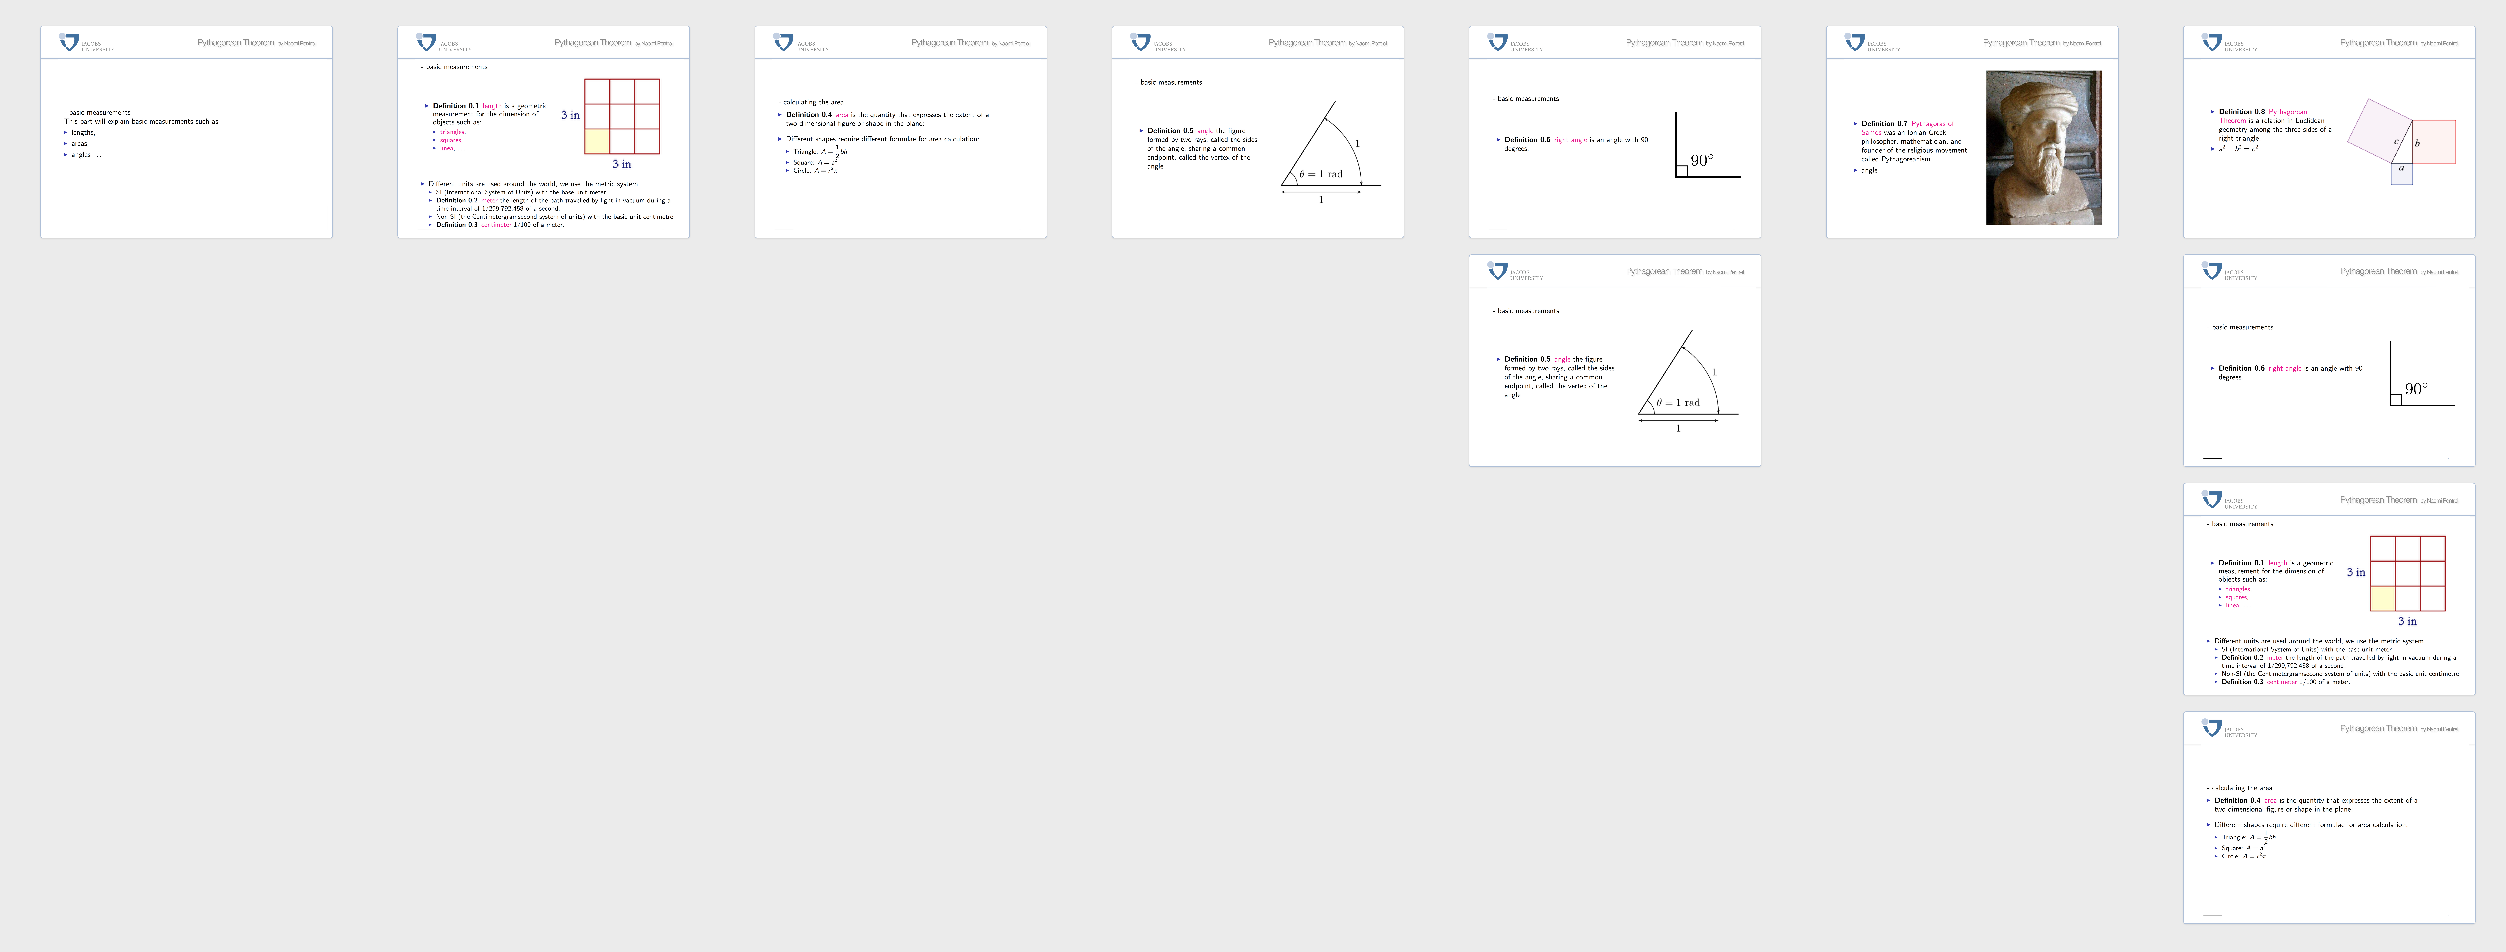
\includegraphics[width=0.87\textwidth]{assets/final/fullPresentation2}
    } 
\vspace{-20pt}
  \caption{Visualization of Dependencies}
  \label{fig:visualDependency}
\vspace{12pt}
  \end{center}
\end{wrapfigure}

\begin{wrapfigure}{c}{\textwidth}
\vspace{-50pt}
\end{wrapfigure}

The library impress.js normally does not support having different paths depending on pressing the right or down key. Therefore it had to be slightly adapted to handle this behavior. As these are implementation details, this will not be further explained here. The interested reader is encouraged to look at the code \cite{npentrel:npentrel15} directly.

\subsection{Levels}
\label{sec:levels}

When writing a document or course notes in \stex, the creator general writes a top-level file such as \textit{notes.tex} from where other \TeX\ files are included. These included files again include further \TeX\ files etc.. Thus we are automatically provided with levels that we can use for splicing our primary narrative path into smaller narrative paths. In essence, on any level the order of information in that topic is a narrative path itself. Expressed in mathematical notation a level within a directed graph $G = \langle V, E \rangle $, with $V$ being a set of nodes and $E = V \times V$ being the set of directed edges, is the set $L_w = \lbrace v \vert \langle w, v \rangle \in E \rbrace$. From these levels we can infer the status of the information. We already know that a dependent piece of information infers that it is \textit{course-ancient} information. Anything that is on the same level or in the sublevels thereof is considered to be \textit{course-old} information.

\begin{wrapfigure}{c}{\textwidth}
\vspace{-16pt}
  \begin{center}
  \fbox{
      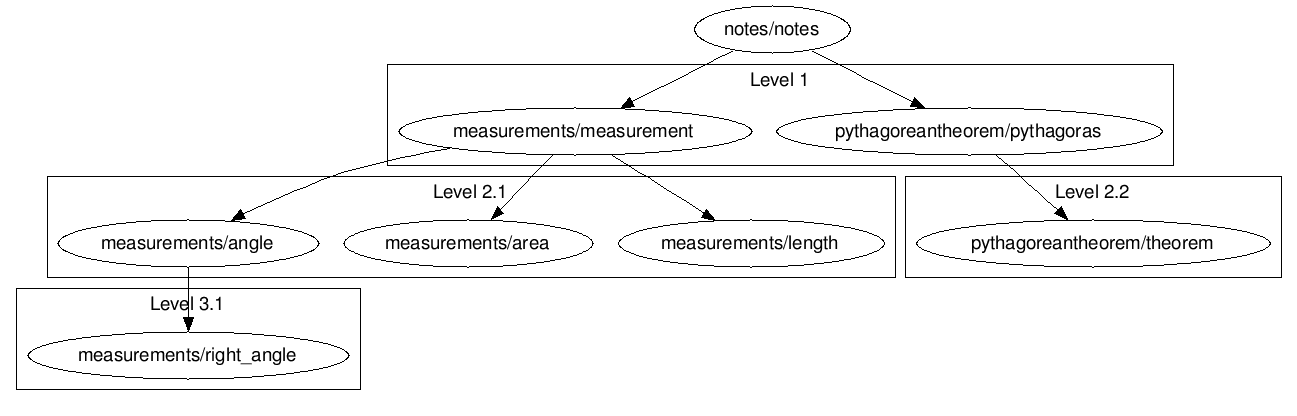
\includegraphics[width=0.97\textwidth]{assets/final/levels}
    } 
\vspace{-20pt}
  \caption{Inclusion Graph with Levels}
  \label{fig:levelsGraph}
\vspace{0pt}
  \end{center}
\end{wrapfigure}

\begin{wrapfigure}{c}{\textwidth}
\vspace{-70pt}
\end{wrapfigure}

If Annie, while browsing through the different dependencies, realizes that she needs to refresh her memory or learn more about any of the dependent information she can enter the respective level. The presentation will then continue on that level and show all the slides from that topic in the correct order. Once Annie has gone through this short excursion, she can return to the initial slide and resume the primary narrative path. By adding a way to explore these other levels, the presentation adds more context and allows Annie to understand the subject on a deeper level. These modular excursions are included in the presentation in 3D by making use of CSS3-transitions (see \autoref{fig:dependencyLevelSnippet}). Thus when the user enters an excursion a 90\degree\ rotation around the y-axis occurs and the user can now follow that story line (see \autoref{fig:visualDependencyDegree}).

\begin{wrapfigure}{r}{\textwidth}
\vspace{-22pt}
\begin{minted}[linenos=true, bgcolor=bg]{C}
<div class="step slide" data-x="8750" data-y="0" data-z="0"
	data-rotate-y="0"> Slide </div>
<div class="step slide" data-x="8750" data-y="800" data-z="0" 
	data-rotate-y="0"> Dependency 1  </div>
<div class="step slide" data-x="8750" data-y="800" data-z="0" 
	data-rotate-y="90"> Dependency 1 Continuation 1 </div>
<div class="step slide" data-x="8750" data-y="800" data-z="1250" 
	data-rotate-y="90"> Dependency 1 Continuation 2 </div>
\end{minted}
\vspace{-8pt}
  \caption{Code Snippet for a Dependency Level}
  \label{fig:dependencyLevelSnippet}
  \vspace{12pt}
\end{wrapfigure}

\begin{wrapfigure}{c}{1\textwidth}
\vspace{-26pt}
  \begin{center}
  \fbox{
      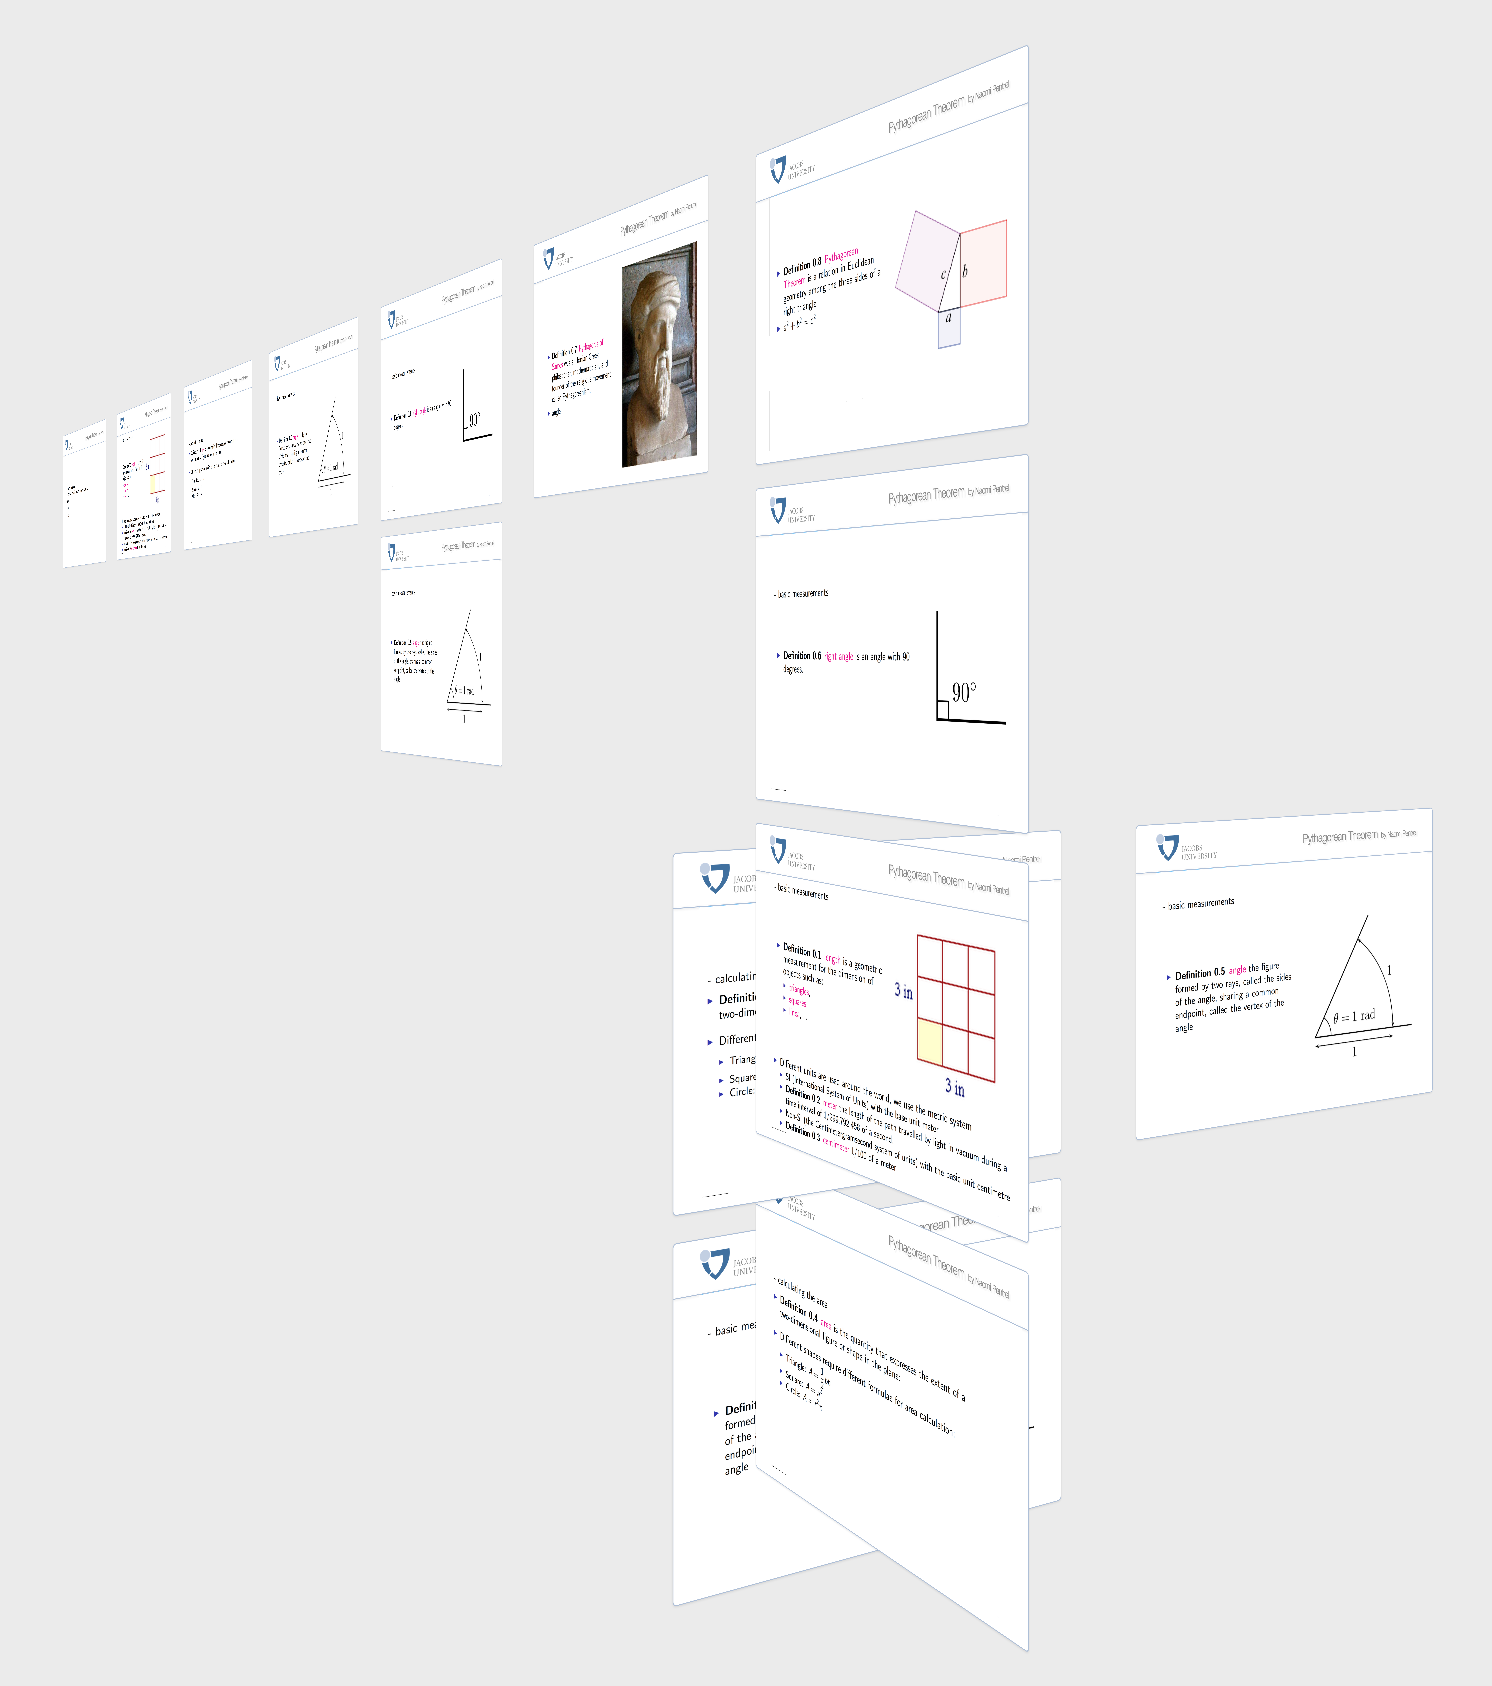
\includegraphics[width=0.65\textwidth]{assets/final/60degree}
    } 
\vspace{-5pt}
  \caption [Caption for LOF]{Visualization of Dependencies and Levels at 60\degree\ \footnotemark}
  \label{fig:visualDependencyDegree}
\vspace{-24pt}
  \end{center}
\end{wrapfigure}

\begin{wrapfigure}{c}{\textwidth}
\vspace{-50pt}
\end{wrapfigure}

\footnotetext{The overlapping slides do not interfere as they are at a 90\degree\ angle. Therefore when seeing one slide, the other slide will be visible only from the slide. Since a slide is very thin this makes it invisible.}

\subsection{The Relational Presentation}
\label{sec:RelationalPresentations}

Combining the information about narrative paths, dependencies, and levels, we derived an ordered information graph out of which we have built a presentation that Annie can interact with to learn about the Pythagorean theorem. In this section we will examine the structure of the created presentation.\\

To begin with, let us examine the choice of layout. The goal of this presentation is to have all the information the Pythagorean theorem depends on easily accessible so that Annie can reach \textit{course-ancient} information easily. The added expressiveness that impress.js offers allowed us to have this in a very structured format. Since Prezi was mentioned in the beginning of this paper as a commercial alternative that was considered for this project, let us examine a sample prezi from afar and outline some differences.\\

\begin{wrapfigure}{l}{0.45\textwidth}
\vspace{-26pt}
  \begin{center}
  \fbox{\href{http://prezi.com/i-bhj8xahg3u/?utm_campaign=share&utm_medium=copy&rc=ex0share}{
      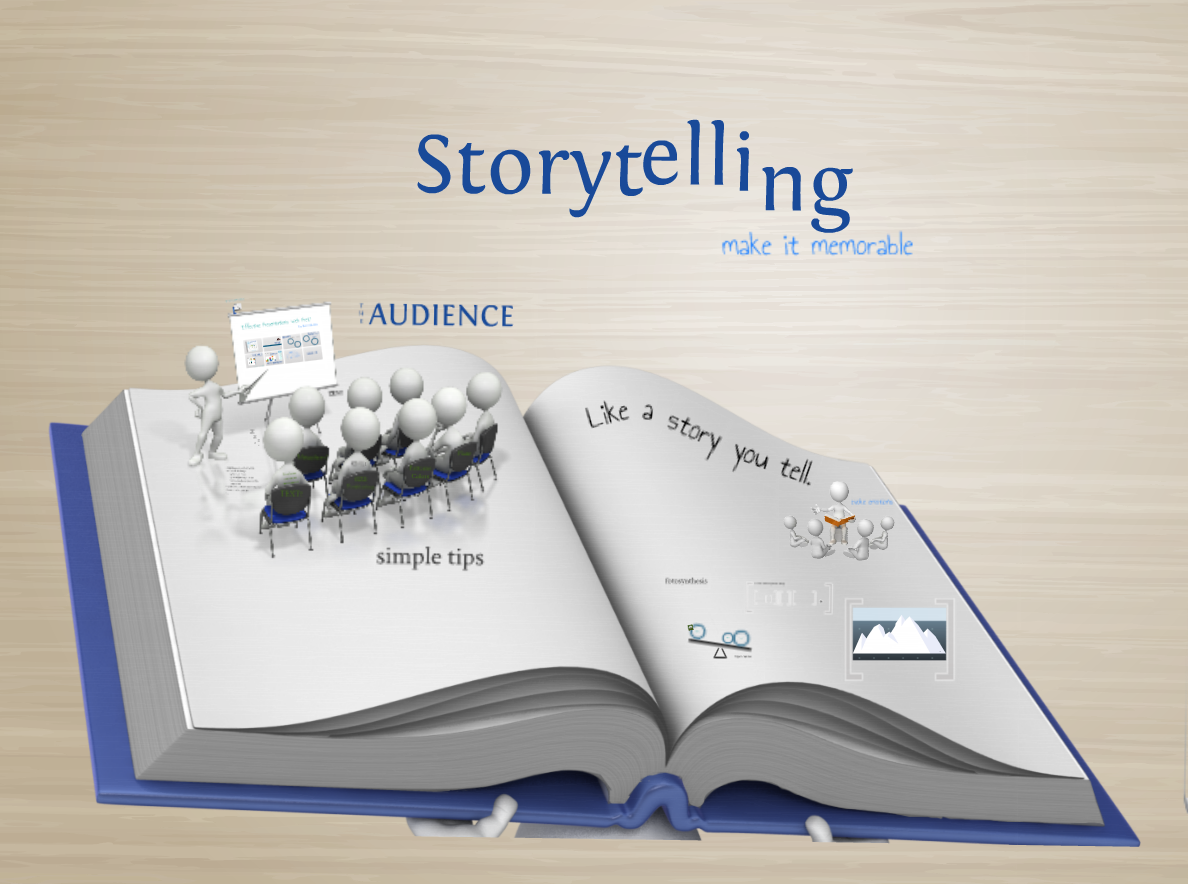
\includegraphics[width=0.42\textwidth]{assets/final/Storytelling}
    } }
\vspace{-20pt}
  \caption{Prezi Example \cite{npentrel2:npentrel15}}
  \label{fig:preziExample}
\vspace{-24pt}
  \end{center}
\end{wrapfigure}

A prezi, if done right, is generally full of metaphors and meaningful visual connections. Our tool cannot mimic this creativity as it lacks the capability to abstract on such a high level. Therefore our product is a lot more structured and focused on visualizing relations between content with movement and closeness. This also serves to keep the resulting presentation simple and easily usable.\\

While focusing on closeness and movement, it can use some of the primitives of impress.js (see \autoref{sec:primitives}) to create meaningful visual relations and semantic movements. These meaningful visual connections are similar to those that prezis often feature. The relations between the content, such as it being the next slide in the narrative or it being a dependency are shown through the closeness and the placement of the slide as well as the movements that come with it. The following movements exist:\\
\vspace{-12pt}
\begin{enumerate}[topsep=0pt,itemsep=-1ex,partopsep=1ex,parsep=1ex]
\item movement along the x-axis,
\item movement along the y-axis, and
\item rotations.
\end{enumerate}
\vspace{5pt}

The movement along the x-axis has a mostly temporal semantics associated with it. Going to the left is connected with going backwards in the narrative, whereas going to the right is associated with going forwards in the narrative. Apart from going forwards and backwards, we can also move along the y-axis. Moving down intuitively means that we dig deeper into a topic and go to the roots of a problem, whereas moving back up means we will be on a higher level.\\

The most interesting movement is the rotations. It should be briefly mentioned that too much rotation leads to seasickness in users, as anyone who has seen a bad prezi can attest to. These are generally rotations around the x-axis that rotate more than 20\degree. Since we only rotate around the y-axis, our rotations are not affected. Instead of causing seasickness, our rotations aim to give the viewer the feeling of entering a topic and a different storyline. Thus entering a different topic comes with a change of perspective which is underlined by the 3D transformation that the user sees. Overall, these movements add expressiveness to the relations and allow for intuitive interaction with the presentation.\\

One might think that this is like a PowerPoint, since PowerPoint offers similar animations to switch slides. The important addition is more obvious when regarding the presentation from a birds perspective by looking at the overview in \autoref{fig:visualDependency} or \autoref{fig:visualDependencyDegree}. The value in these presentations is that through these overviews, dependencies become identifiable. More importantly this means that for Annie, dependencies become accessible and allow her to go on small guided tours or small excursions into \textit{course-ancient} topics giving her the flexibility to choose her own path while going through the presentation.

\section{Evaluation}
\label{sec:eval}

Even though an evaluation is not fully possible given the limited time frame, we will attempt to evaluate the created system and the created presentations as well as their shortcomings. Afterwards we will briefly look at future work and possible extensions to our system.\\

\begin{wrapfigure}{l}{0.35\textwidth}
\vspace{-28pt}
  \begin{center}
  \fbox{
      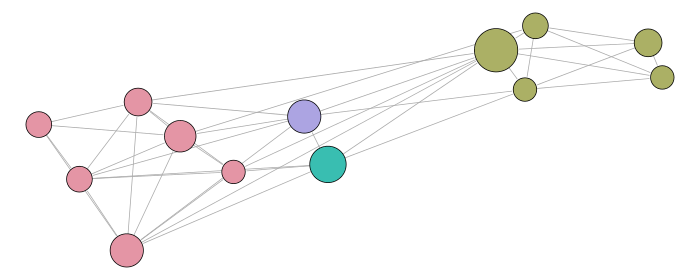
\includegraphics[width=0.33\textwidth]{assets/final/initialIdea}
    }
\vspace{-20pt}
  \caption{Initial Presentation Idea}
  \label{fig:initialIdea}
\vspace{-24pt}
  \end{center}
\end{wrapfigure}

The evaluation conducted in the following part is on the one hand, systematic and, on the other hand, cognitive. Systematically, the knowledge presentation system \sys that was developed allows for the creation of a clearly structured relational presentation from a given annotated document which fulfills the goal of this project. It does so in a very timely manner within seconds. In the starting phase of this research, the created presentations were supposed to look a lot more like clustered graphs such as \autoref{fig:initialIdea}. Possibly with nodes that are close if they are semantically close and the size of the nodes reflecting the importance of the node. While implementing the system, it not only became obvious that such an implementation would be very difficult but also that it would likely confuse our persona, Annie.\\

When using Prezi, it is a human being that can creatively think of links and therefore make more graphical presentations. Due to the fact that our system only has limited intelligence, we end up with a far more structured presentation. However, considering that the goal of the created presentation is to allow users to intuitively understand dependencies and to allow them to deviate from the primary narrative path to enter the level of one of the dependencies and follow its narrative path for a while, it became obvious that a simple structure for this presentation is even preferable.\\

After having considered the systematic aspects, let us now look at the cognitive aspects. Cognitively, we explored a part of the field of information systems. It is still an open question whether the developed system provides a better system for knowledge transfer. I strongly believe that the created system \sys adds value to presentation and has the power to facilitate and improve knowledge transfer due to some reasons that were already shown in the \autoref{sec:relatedworks}. These sources argued that the linking of learning materials is useful for knowledge transfer and that especially mathematics is a field that could profit from guided tours through topics as a way of learning topics according to users' individual knowledge bases.\\

\begin{wrapfigure}{l}{0.35\textwidth}
\vspace{-28pt}
  \begin{center}
  \fbox{\href{http://prezi.com/i-bhj8xahg3u/?utm_campaign=share&utm_medium=copy&rc=ex0share}{
      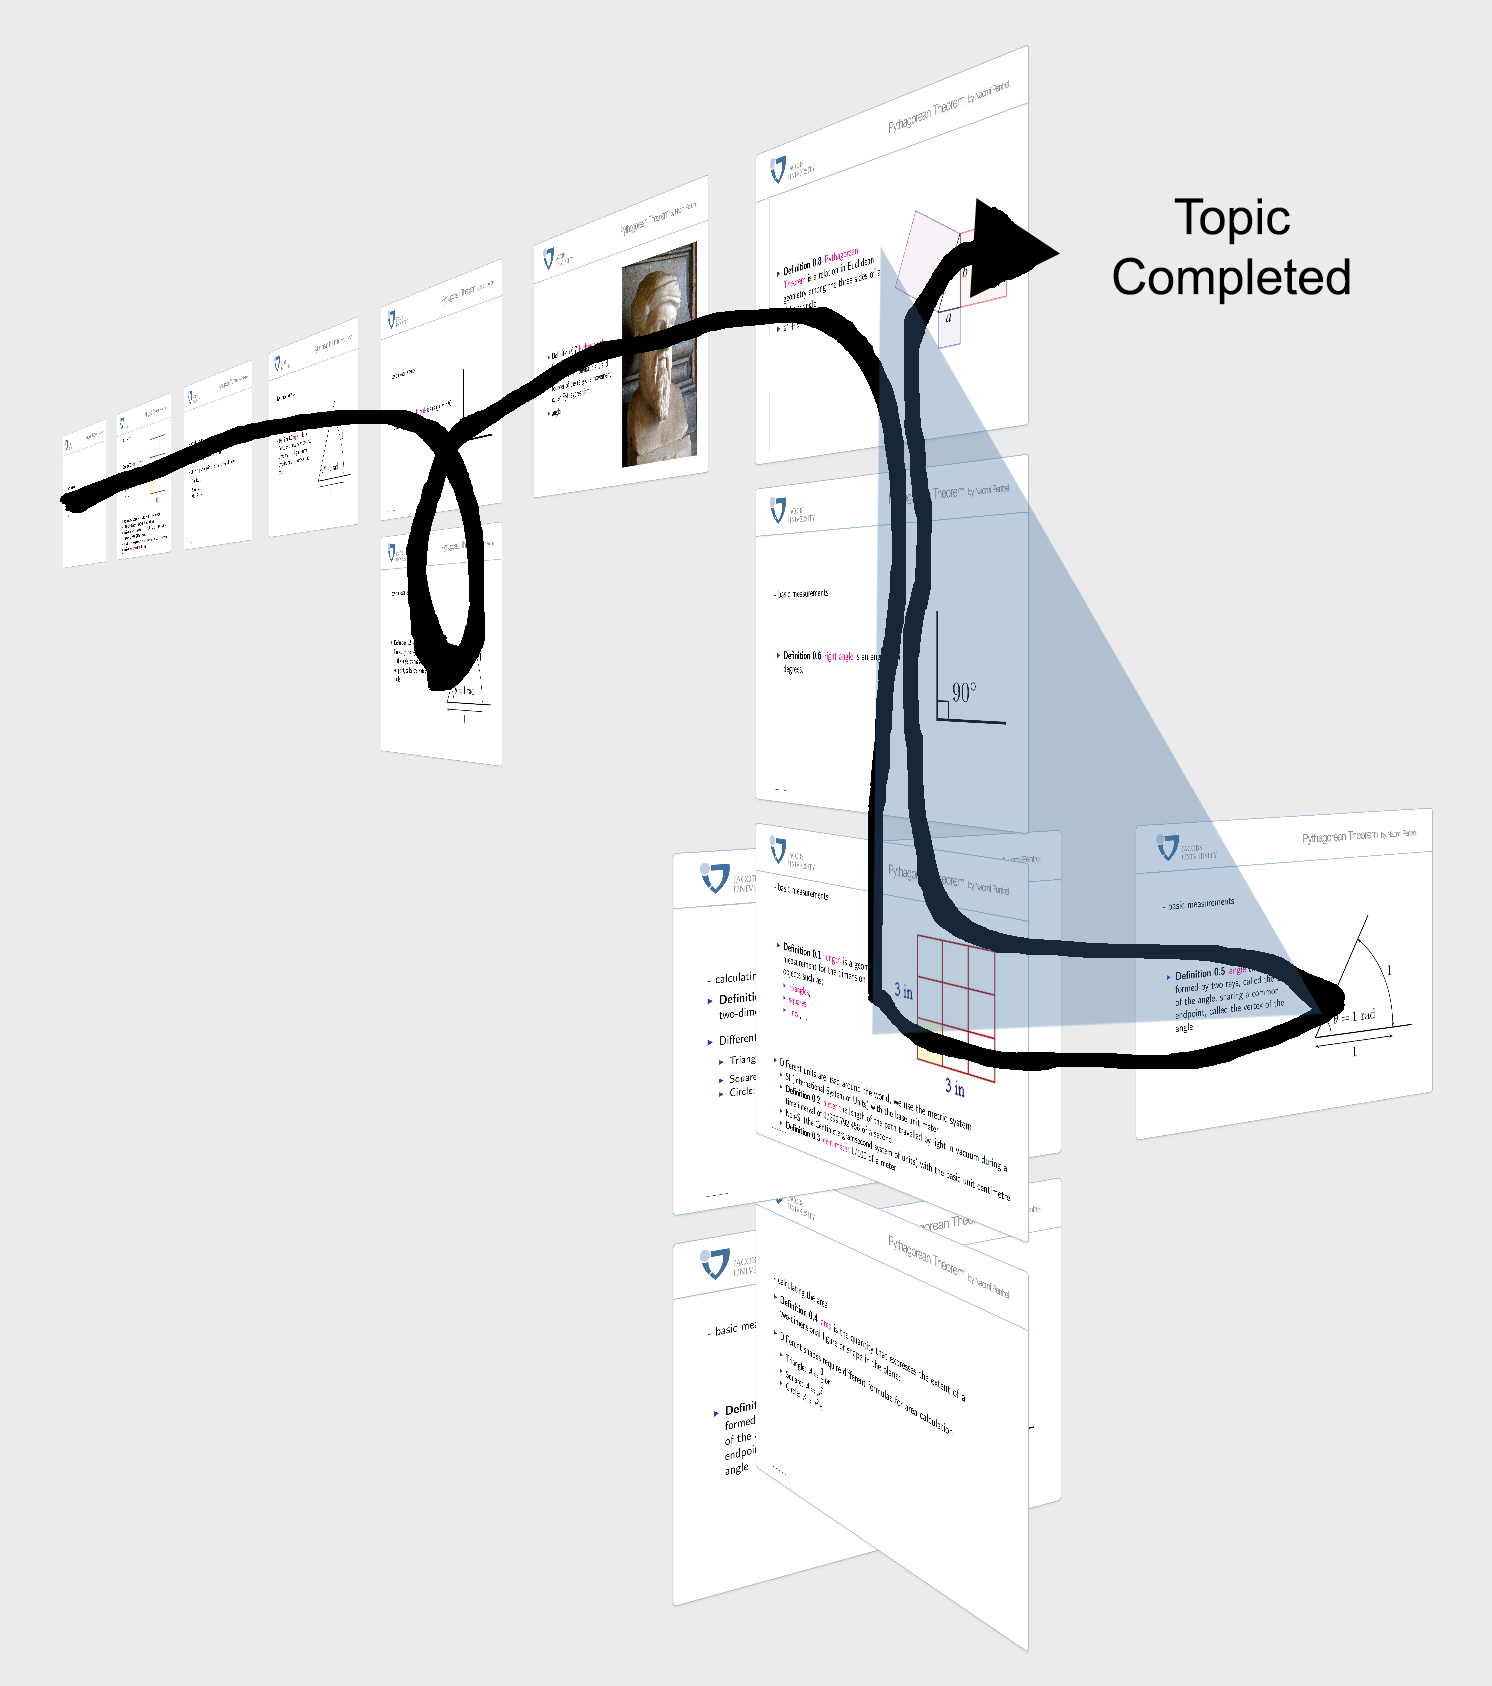
\includegraphics[width=0.33\textwidth]{assets/final/ExamplePathTriangle}
    } }
\vspace{-20pt}
  \caption{Path Example}
  \label{fig:pathExample}
\vspace{-40pt}
  \end{center}
\end{wrapfigure}

Since a qualitative analysis was unfortunately not possible in this time frame, we can only make an educated guess at the usefulness. To strengthen this educated guess, we will look at the potential path a user could take through the presentation we created by examining \autoref{fig:pathExample}.\\

In the book \textit{OMDoc - An Open Markup Format for Mathematical Documents} \cite{URL:omdocspec}, a didactic figure called the straw-man theory is introduced as an example for a na\"{i}ve reduced approximation of the real theory that aims to show an example to explain why said approximation does not work. Our system is not sophisticated enough to examine these structures on its own and figure out which information is best to be shown. Instead, \sys simply finds where the dependent information has been taught before and reuses the order in which it was taught before. Subsequently, our system heavily relies on sensible input.\\

Given this sensible input our persona, Annie can make use of digressions, where she can go back to a different topic and follow its narrative path for a while. An example for this is highlighted with a blue triangle in \autoref{fig:pathExample}. These digressions are the added value that allow flexibility in these new presentation and transform the traditional presentations from linear presentations to relational presentations.


\section{Future Work and Possible Extensions}

This section lists some ideas on future work regarding this topic and the created system \sys. Before embarking on improvements of the system, a qualitative and quantitative analysis of the produced visual presentations should be conducted to confirm that this system helps users. For the quantitative analysis it would be ideal to take a course that has already been taught using a more traditional approach to presentations which can then function as a control group. After teaching the whole course using the newly created presentation, the data of how the students in this test group performed can be compared with the gathered data from how students used to perform in the course. For a qualitative analysis, students who have been subject to the use of and who have actively used the new presentation could be interviewed.\\

Apart from an analysis to evaluate the effectiveness of the created presentations, the whole system could be made more user friendly for both the creator and the users of the presentations. By improving the creation user interface and allowing for users to choose their own designs, it becomes more easy to use and more attractive for users. Adding an editor would make this more user friendly for creators as well. To change a presentation after it has been created, a user currently has to understand how to manipulate HTML, JavaScript, and also CSS.\\

In terms of improving the usability for the users that will view and interact with the presentations, one could try to find a way to make use of relative size to additionally convey importance using impress.js' \texttt{data-scale} attribute. This would further add more semantic meaning to the slides. Additionally, one could think about adding a progress bar by using the work of Matthias Bilger \cite{bilger:npentrel15} to motivate users to continue.\\

Overall it is even thinkable to create a different version of this system that could be made available to common users outside this research domain. The idea would be to allow users to add slides in an editor and to allow them to add dependencies themselves. Possibly the system could even suggest dependencies. As an example, I could very well envision a biology presentation that explains photosynthesis and allows the attentive student to catch up on dependencies such as the process that transforms ADP to ATP.\\

In terms of improving content, it would be interesting to not just provide paths to dependencies or prerequisite knowledge but also to knowledge that builds on the current topic. That way students that learn fast can already explore higher levels.\\

This whole research project might also benefit from machine learning which could allow us to make smart offers of likely dependencies. On an individual basis we could use it to learn what the user knows and what the user does not know. Ideally we do not always want to show very low level dependencies, such as how to multiply, which our system could then learn. Combining machine learning with the identification of more didactic paths or figures within the data such as the example in \autoref{fig:pathExample} could further improve knowledge transfer.

\section{Conclusion}
\label{sec:conclusion}

In this research project we set out to help Annie understand the Pythagorean theorem. Her problem was that she did not know about some of the dependent information, i.e. right angles, and since there was no easy way to access this information she could not understand the topic fully. To help her, we created a system \sys that parses the documents that the instructor wrote and created a relational presentation out of it.\\

This relational presentation combines spatial narrative with information about the relations between different pieces of information into a visual information graph. In doing so it creates presentations that use meaningful visual connections between pieces of information to allow for intuitive interaction with the presentation. This allows Annie choose her own path in going through the presentation while seamlessly looking up related information.\\

The benefits are not just for Annie when she is going through the presentation on her own, though, Annie's teacher now has a tool that allows him to use his normal lecture material in a more interactive way. Thus when the teacher realizes that the students need to revise previous material, the teacher can seamlessly go to that material and provide them with a good learning experience. This facilitates knowledge transfer and allows for a more engaging and interactive education.\\

In the future, I believe that this research could be adopted in more fields, transforming education into something that allows individuals to learn the way that is best for them. In the introduction, I introduced the metaphor of hiking up a mountain which can be done in different ways. The type of presentations this research built allows for a lot of different paths to reach a learning goal. The flexibility that comes with these presentations is undoubtedly preferable to traditional presentations as it offers clear benefits in allowing to effortlessly change the path of the presentation at any point.\\


\newpage

\bibliography{kwarc}{}
\bibliographystyle{alpha}
\end{document}
